\chapter{IOZone benchmarking diagrams}
This appendix contains all figures of the IOZone benchmarking outputs produced. Each section contains the figures for the benchmarking results of the specific filesystem. Each figure represents one IOZone test, and each graph in the figures visualizes the performance of the filesystem for different file sizes. The x-axis shows the buffer size in kilobytes, and the y-axis is the throughput in kilobytes per second.

\section{FFS}
\begin{figure}[!htb]
	\label{fig:app_bench_ffs_rnd_read}
	\begin{center}
		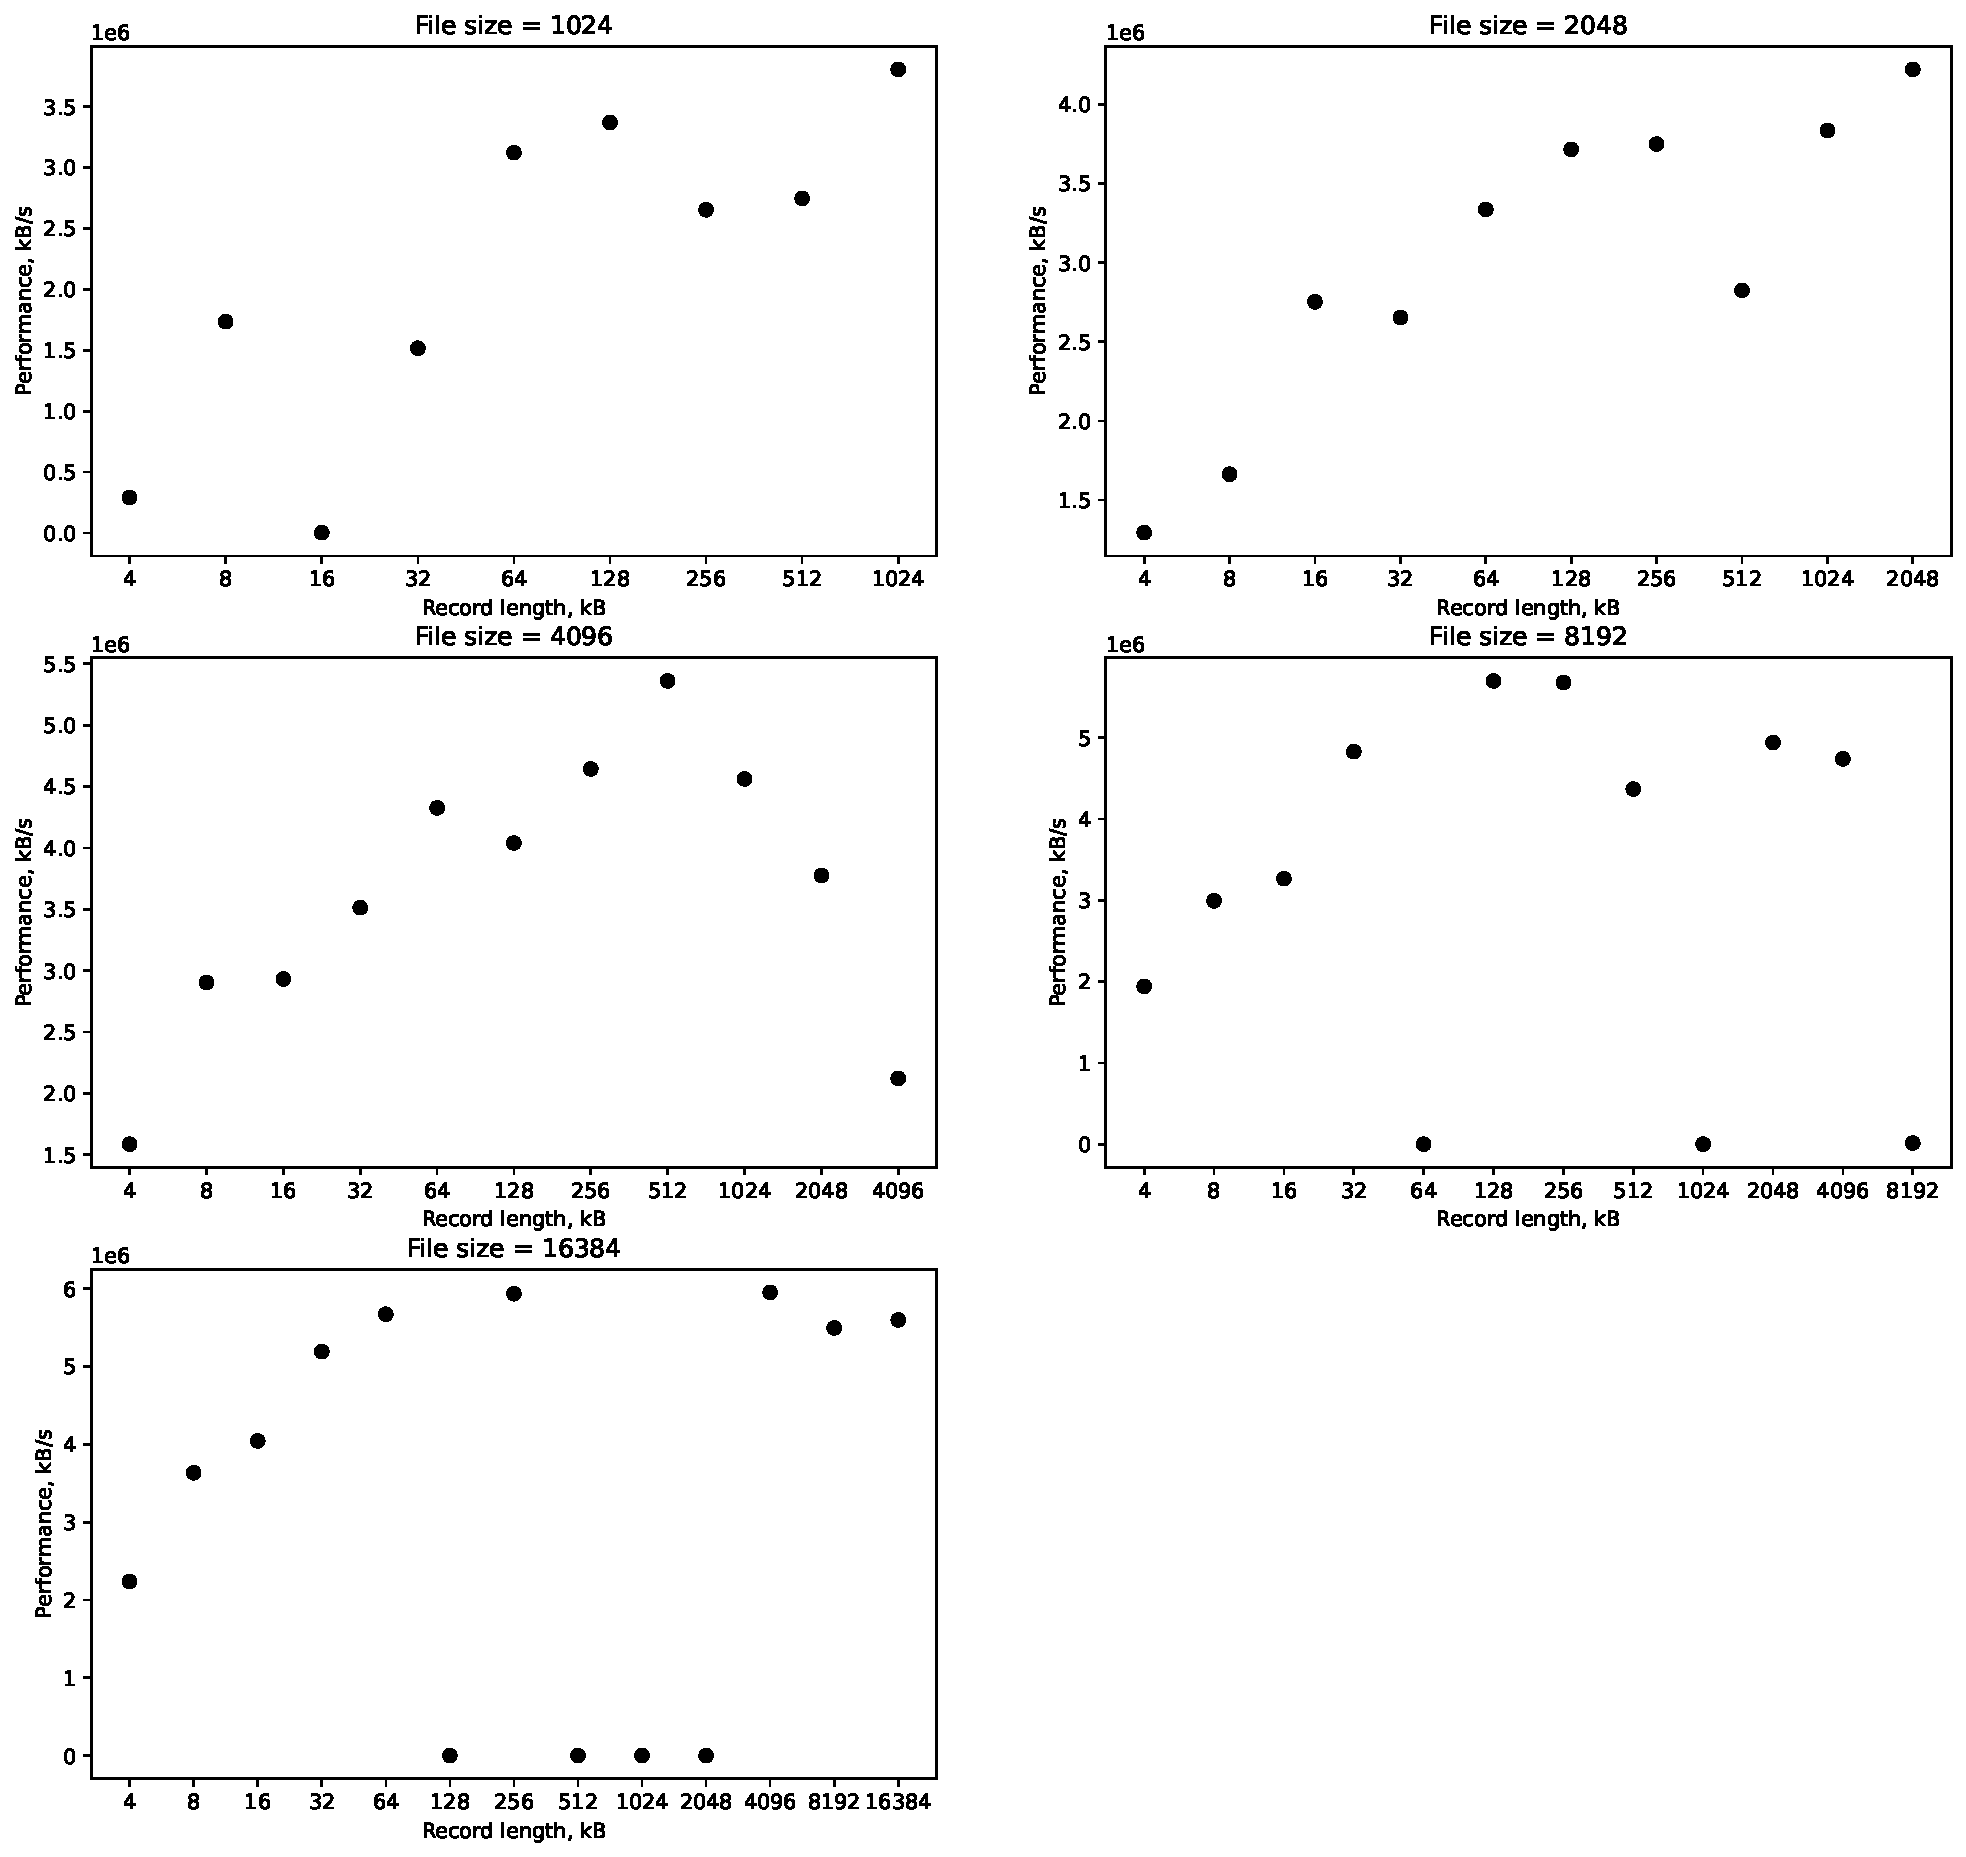
\includegraphics[width=1.0\textwidth]{figures/benchmarking/ffs/Reader.pdf}
	\end{center}
	\caption{IOZone output for FFS Forward Read}
\end{figure}

\begin{figure}[!htb]
	\label{fig:app_bench_ffs_rnd_read}
	\begin{center}
		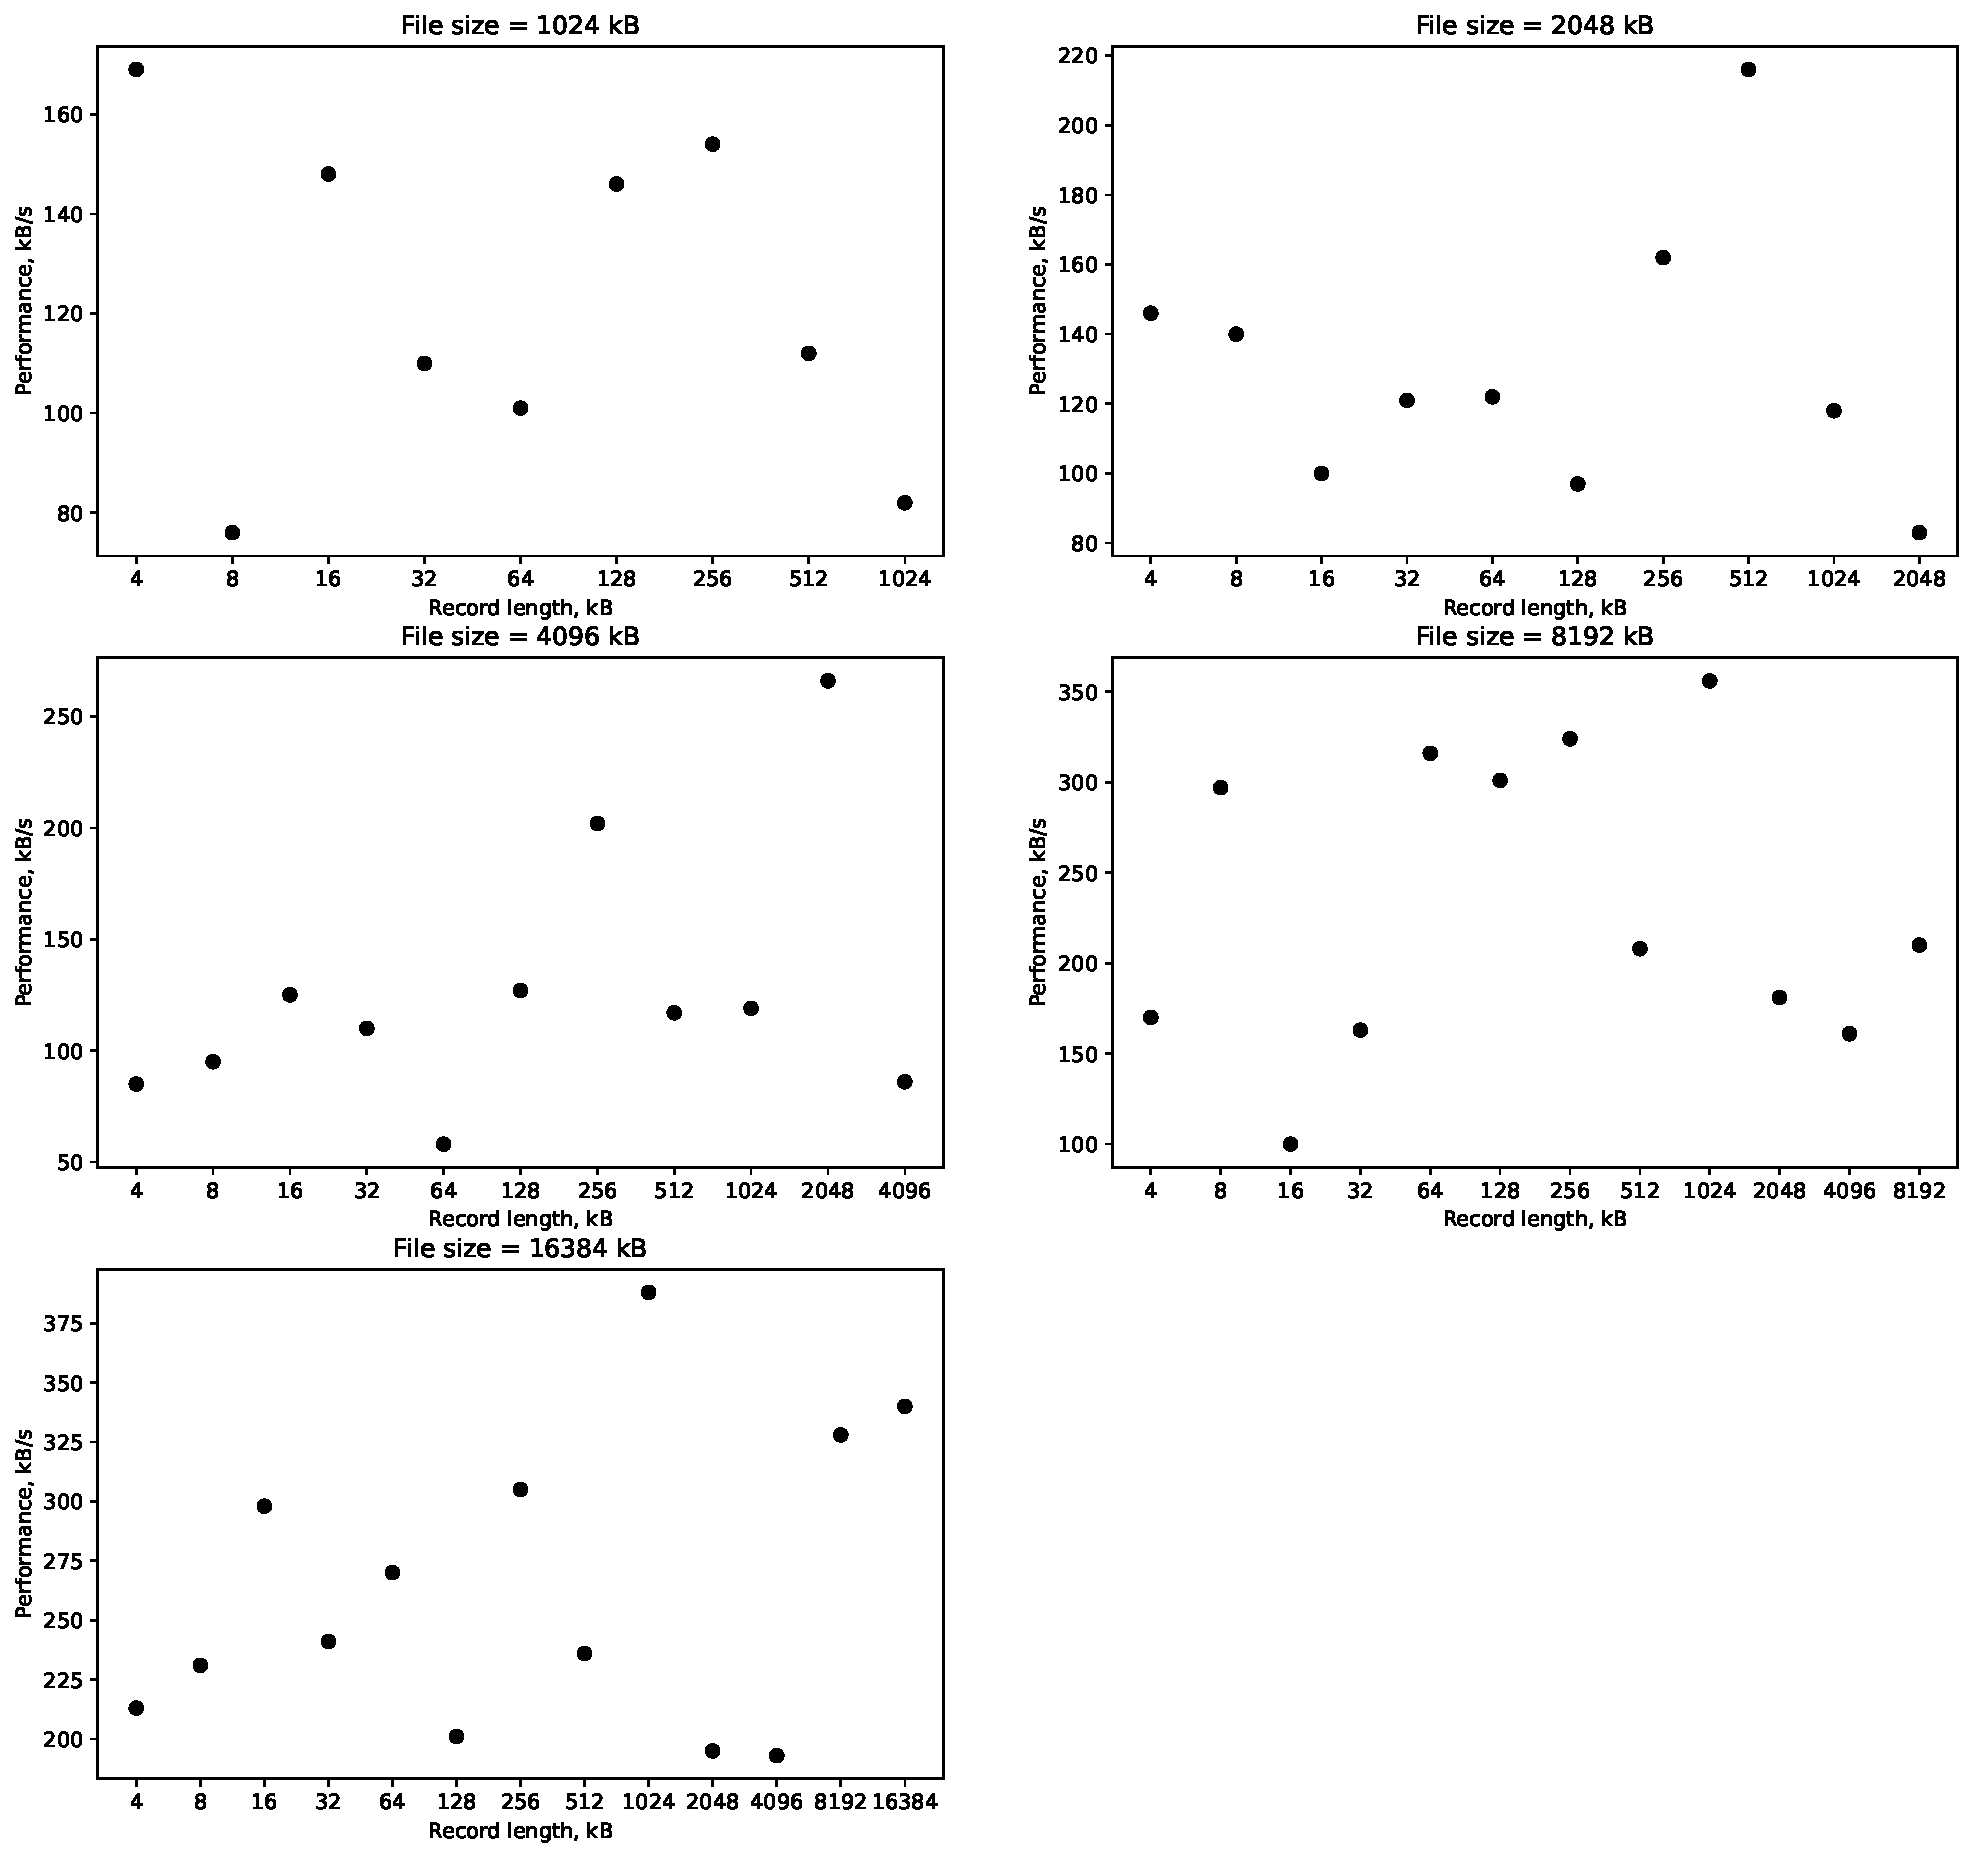
\includegraphics[width=1.0\textwidth]{figures/benchmarking/ffs/Writer.pdf}
	\end{center}
	\caption{IOZone output for FFS Forward Write}
\end{figure}

\begin{figure}[!htb]
	\label{fig:app_bench_ffs_rnd_read}
	\begin{center}
		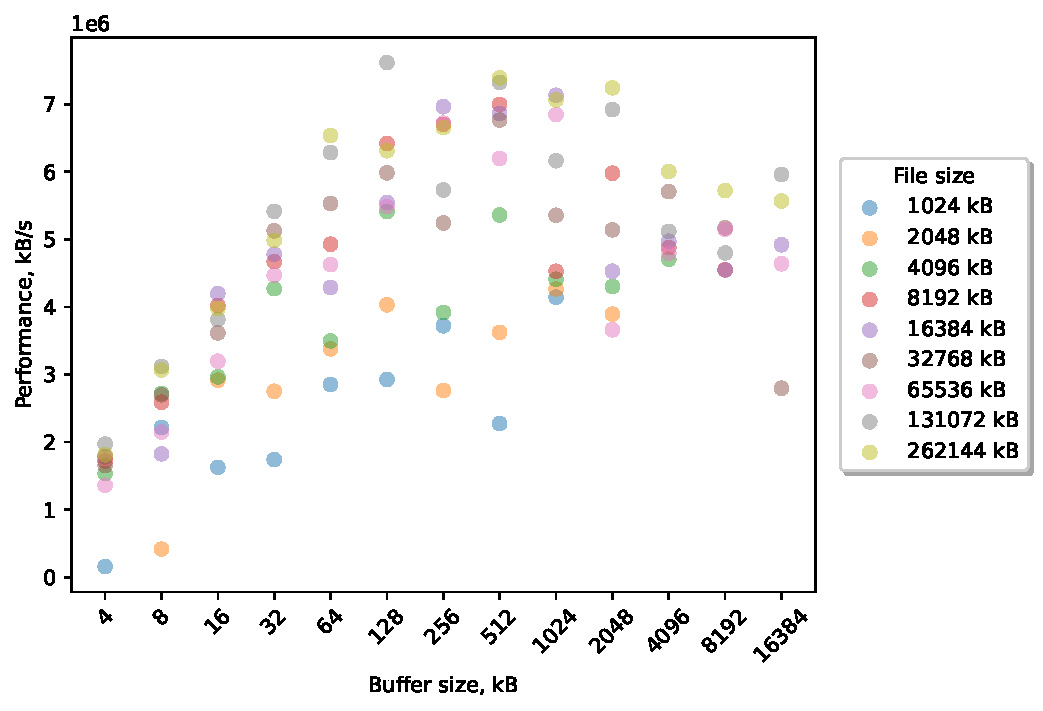
\includegraphics[width=1.0\textwidth]{figures/benchmarking/ffs/Random read.pdf}
	\end{center}
	\caption{IOZone output for FFS Random read}
\end{figure}

\begin{figure}[!htb]
	\label{fig:app_bench_ffs_rnd_read}
	\begin{center}
		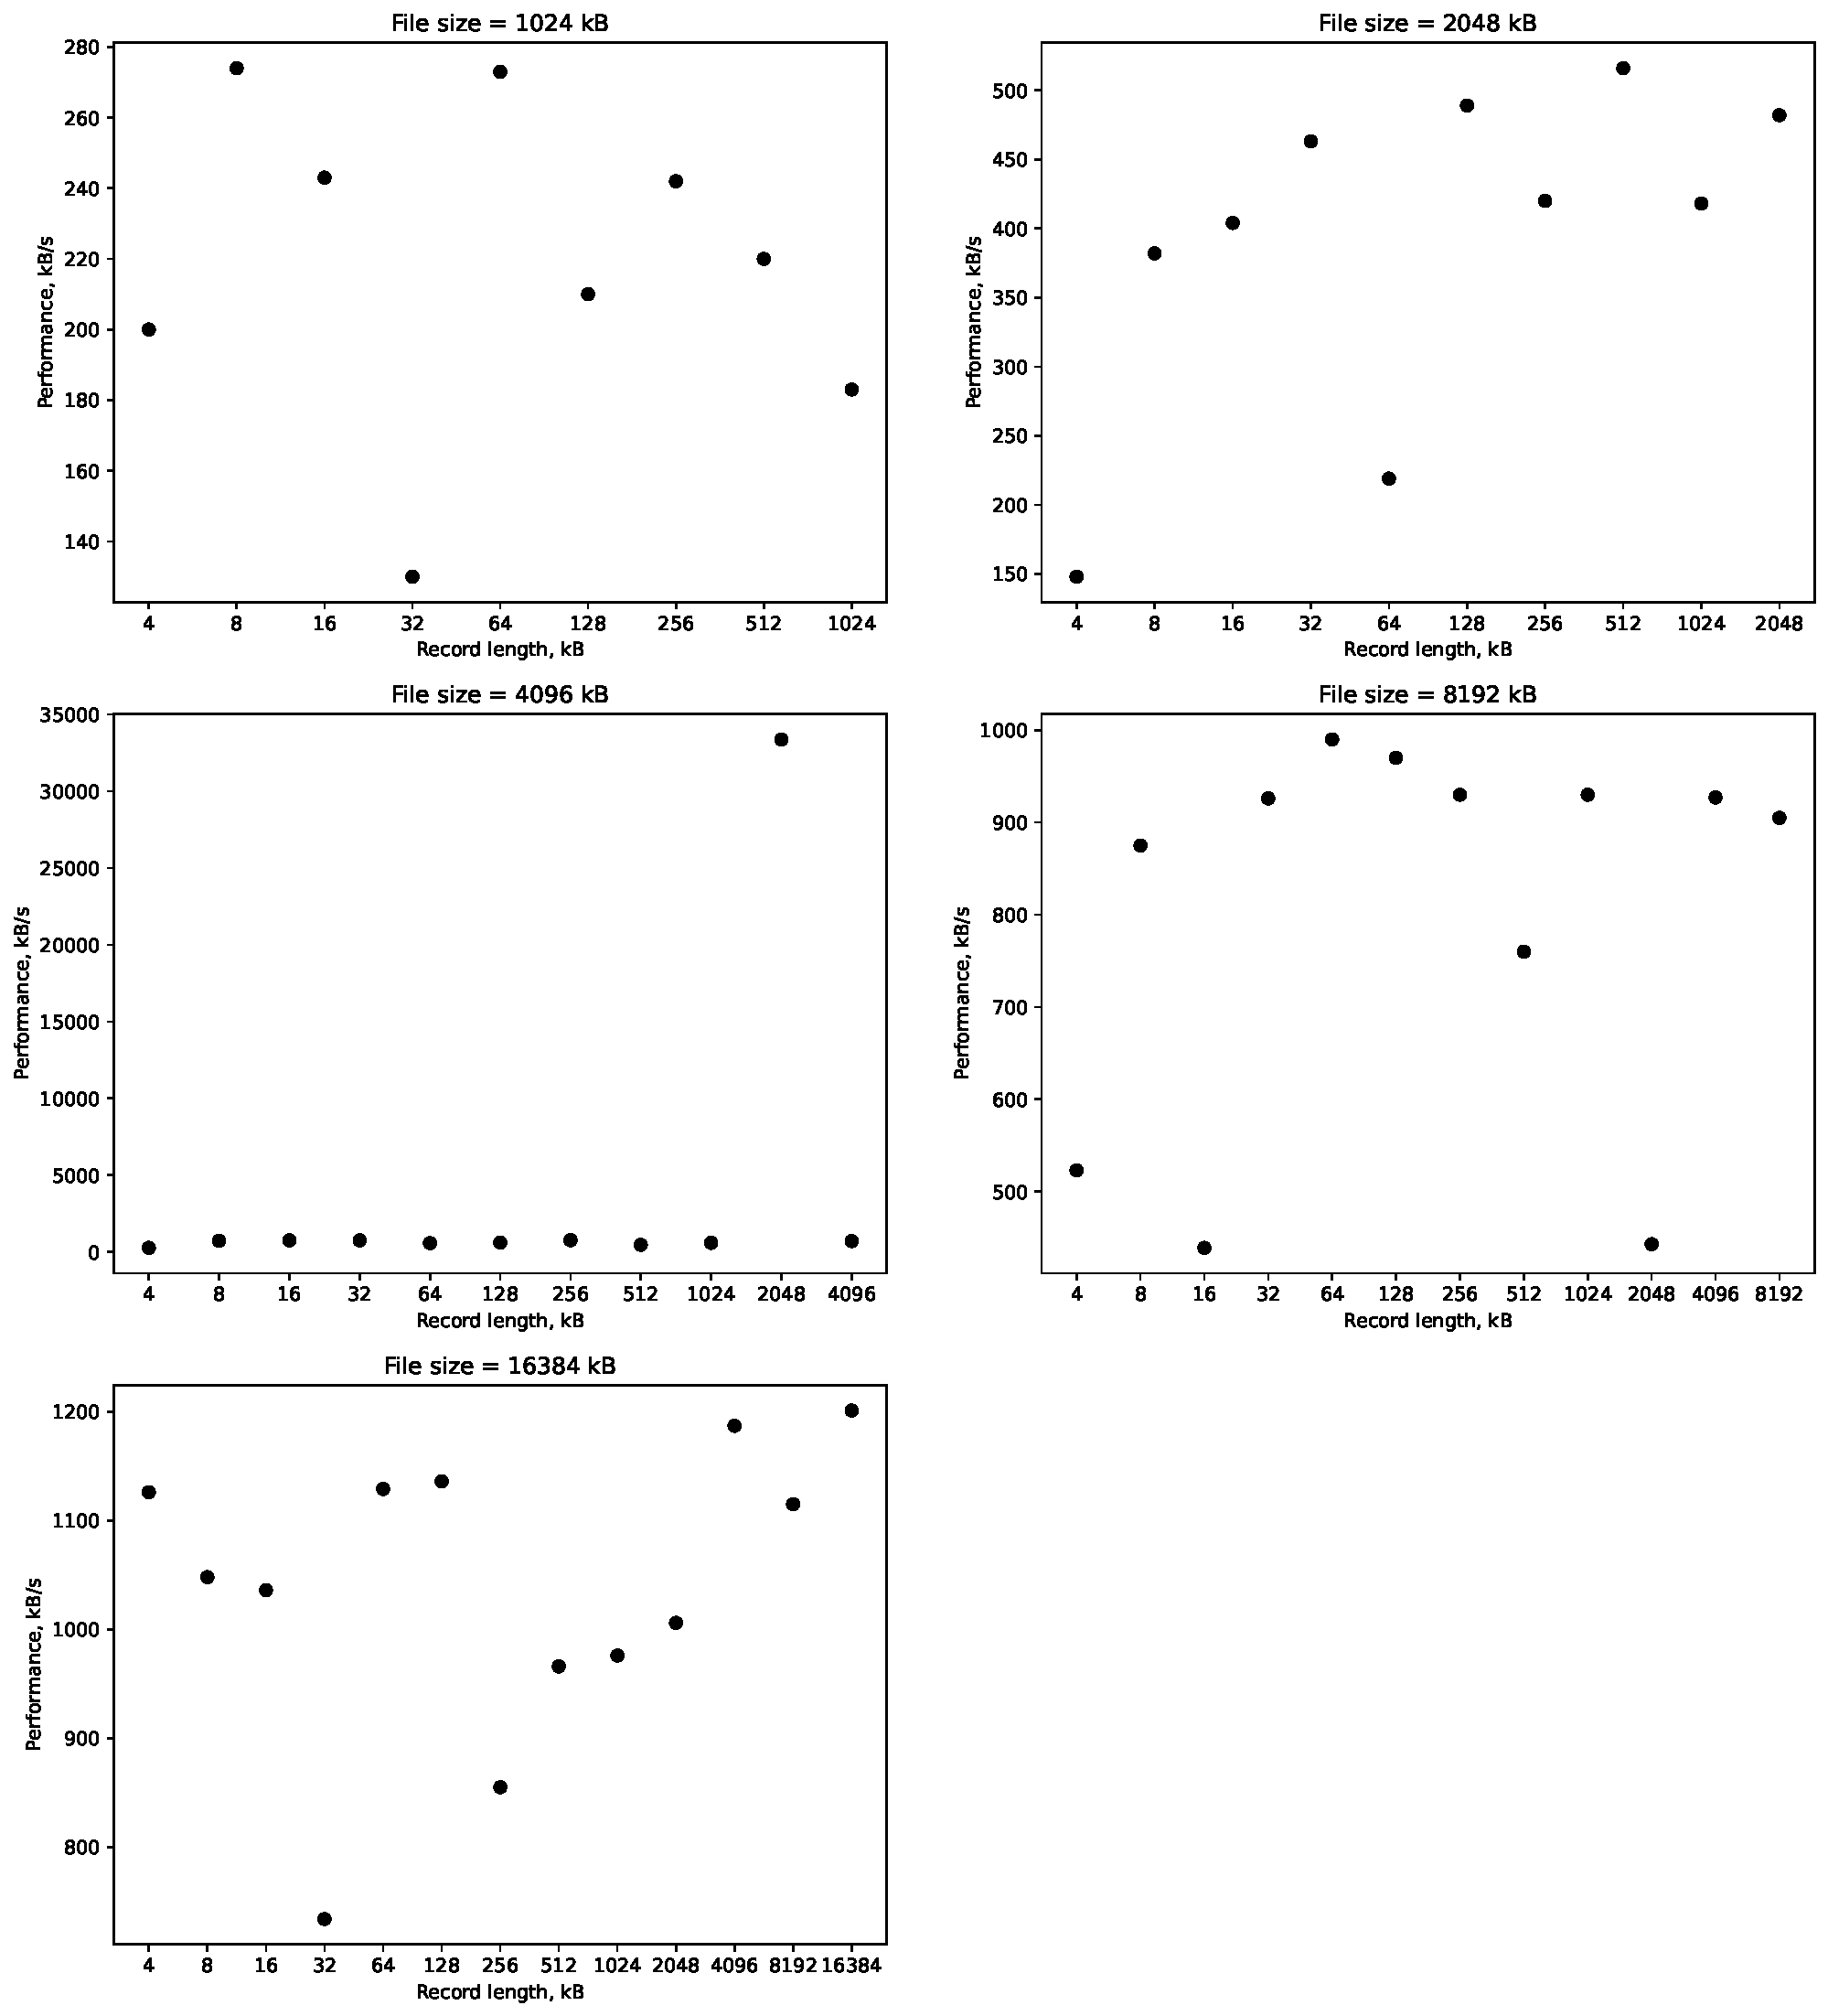
\includegraphics[width=1.0\textwidth]{figures/benchmarking/ffs/Random write.pdf}
	\end{center}
	\caption{IOZone output for FFS Random write}
\end{figure}

\begin{figure}[!htb]
	\label{fig:app_bench_ffs_rnd_read}
	\begin{center}
		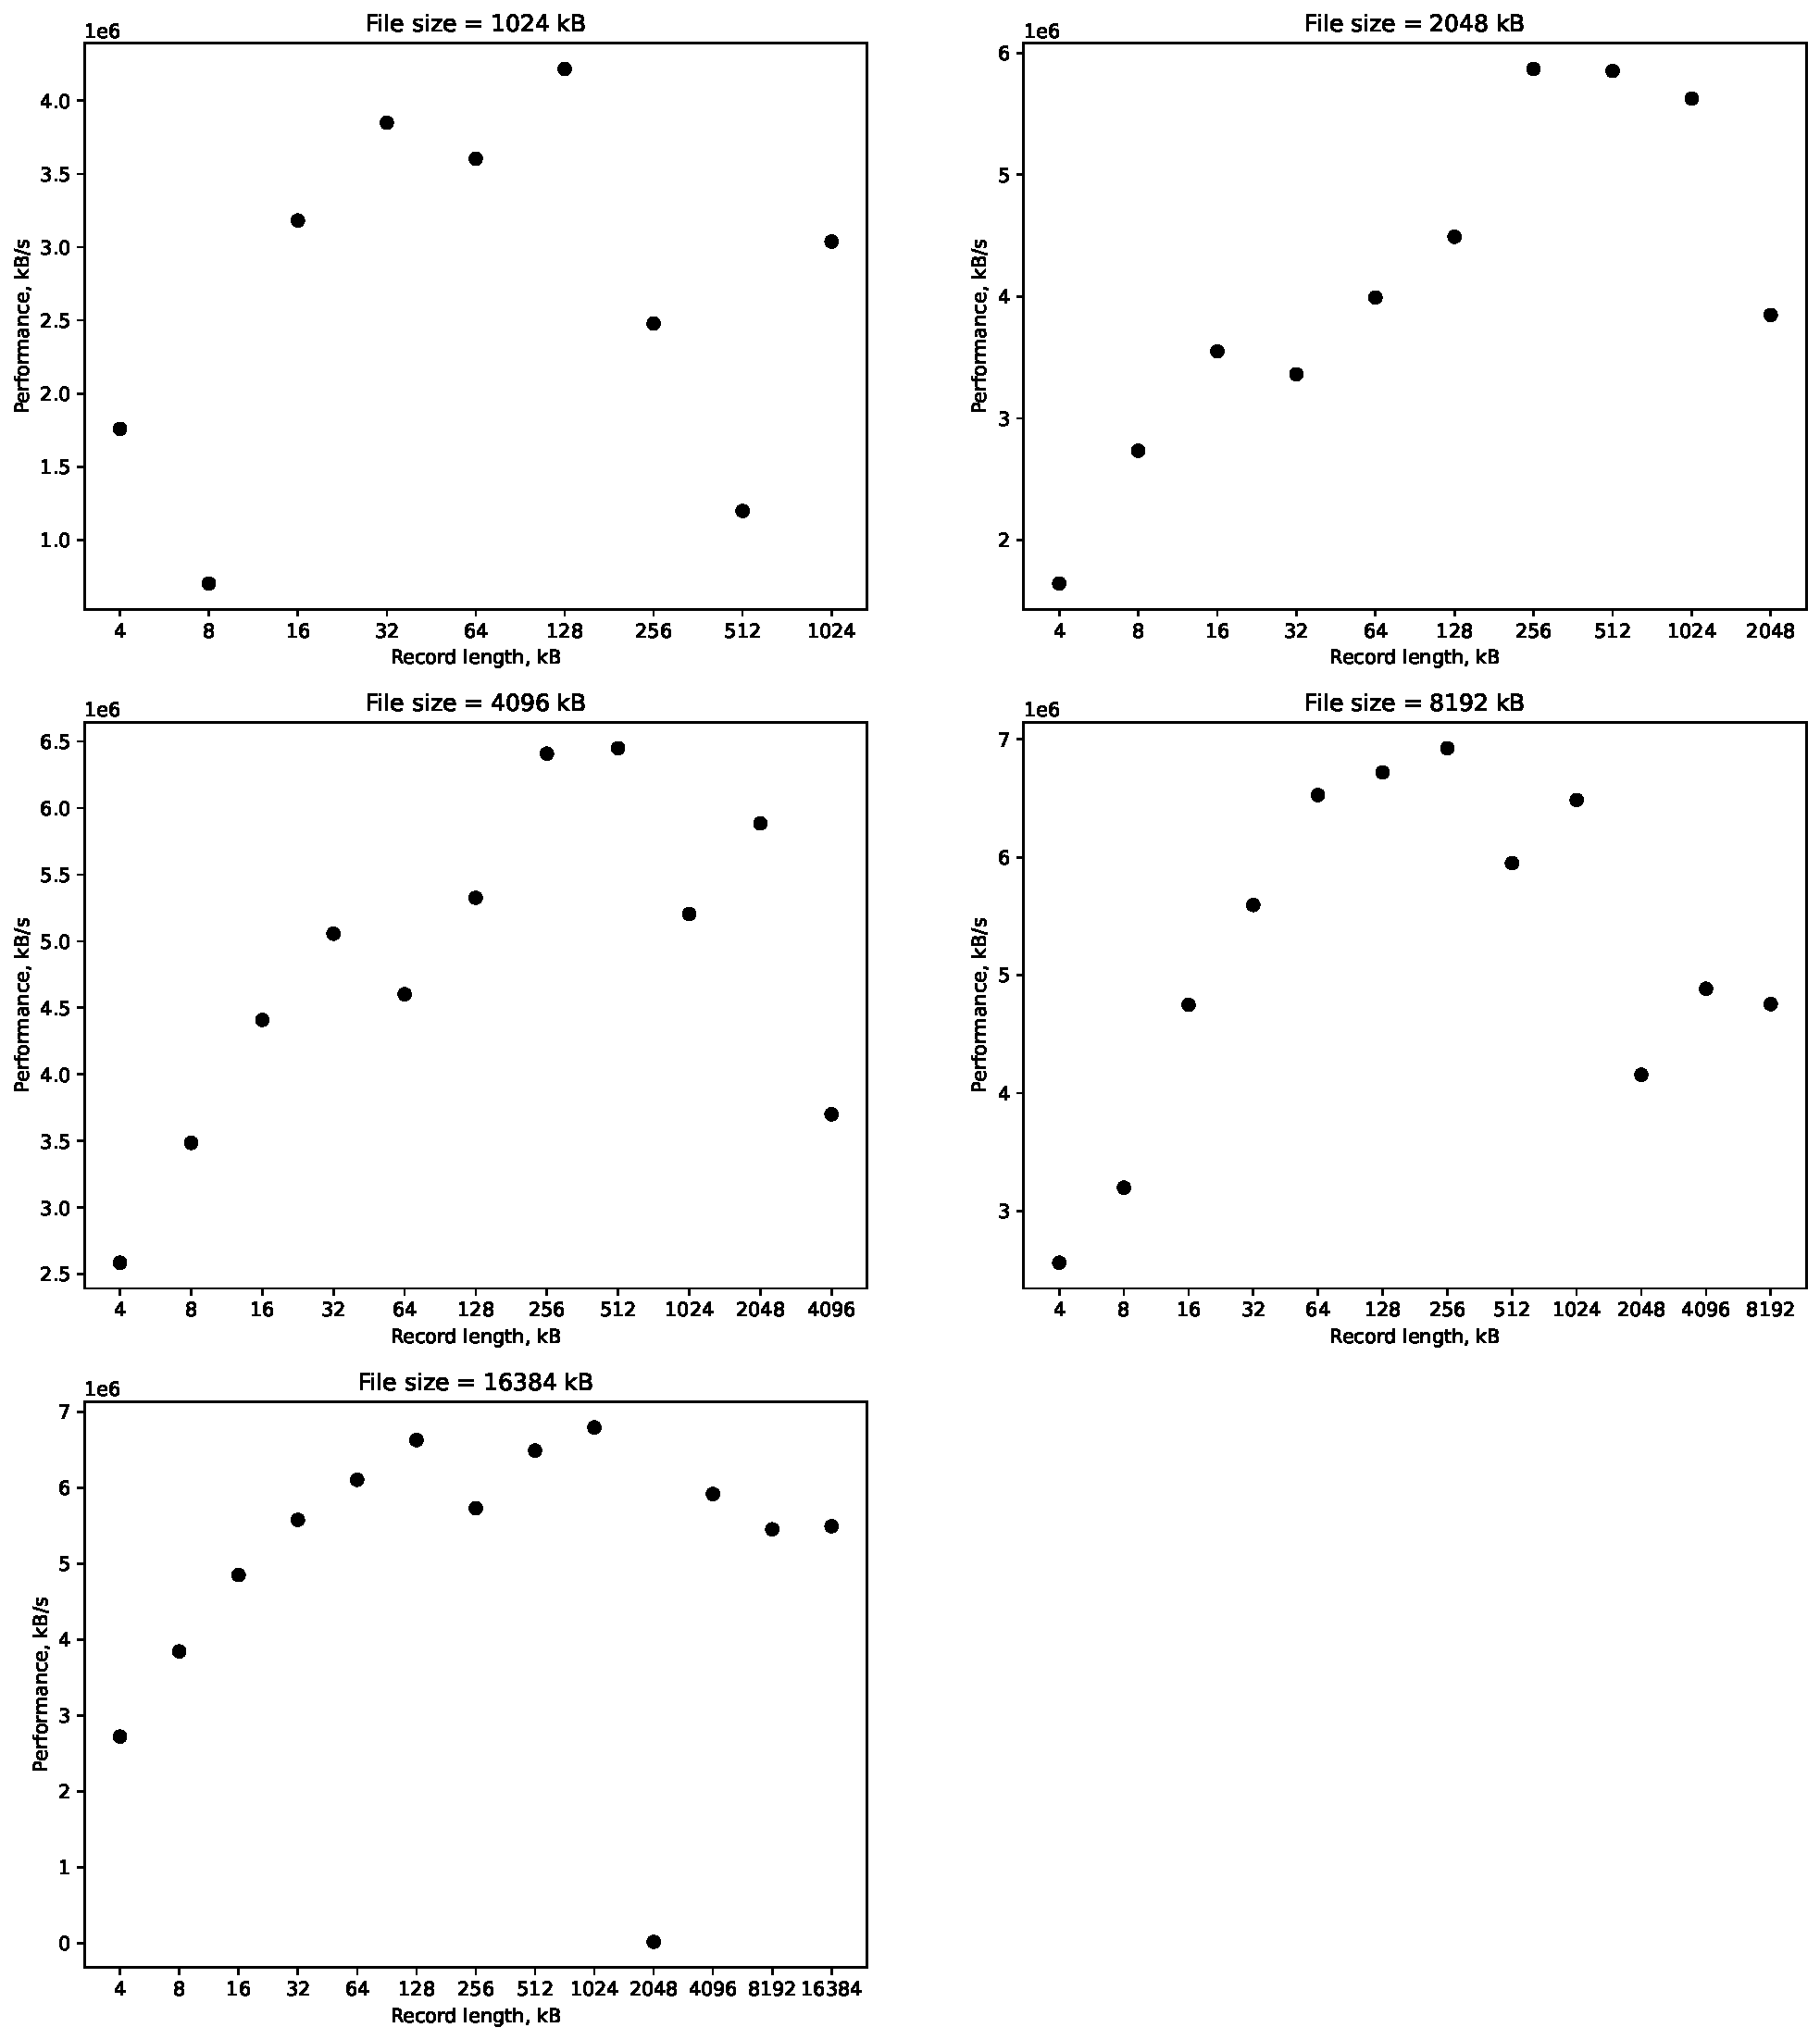
\includegraphics[width=1.0\textwidth]{figures/benchmarking/ffs/Re-Reader.pdf}
	\end{center}
	\caption{IOZone output for FFS Re-Read}
\end{figure}

\begin{figure}[!htb]
	\label{fig:app_bench_ffs_rnd_read}
	\begin{center}
		\includegraphics[width=1.0\textwidth]{figures/benchmarking/ffs/Re-Writer.pdf}
	\end{center}
	\caption{IOZone output for FFS Re-Write}
\end{figure}


\section{Fake FFS}
\begin{figure}[!htb]
	\label{fig:app_bench_fffs_rnd_read}
	\begin{center}
		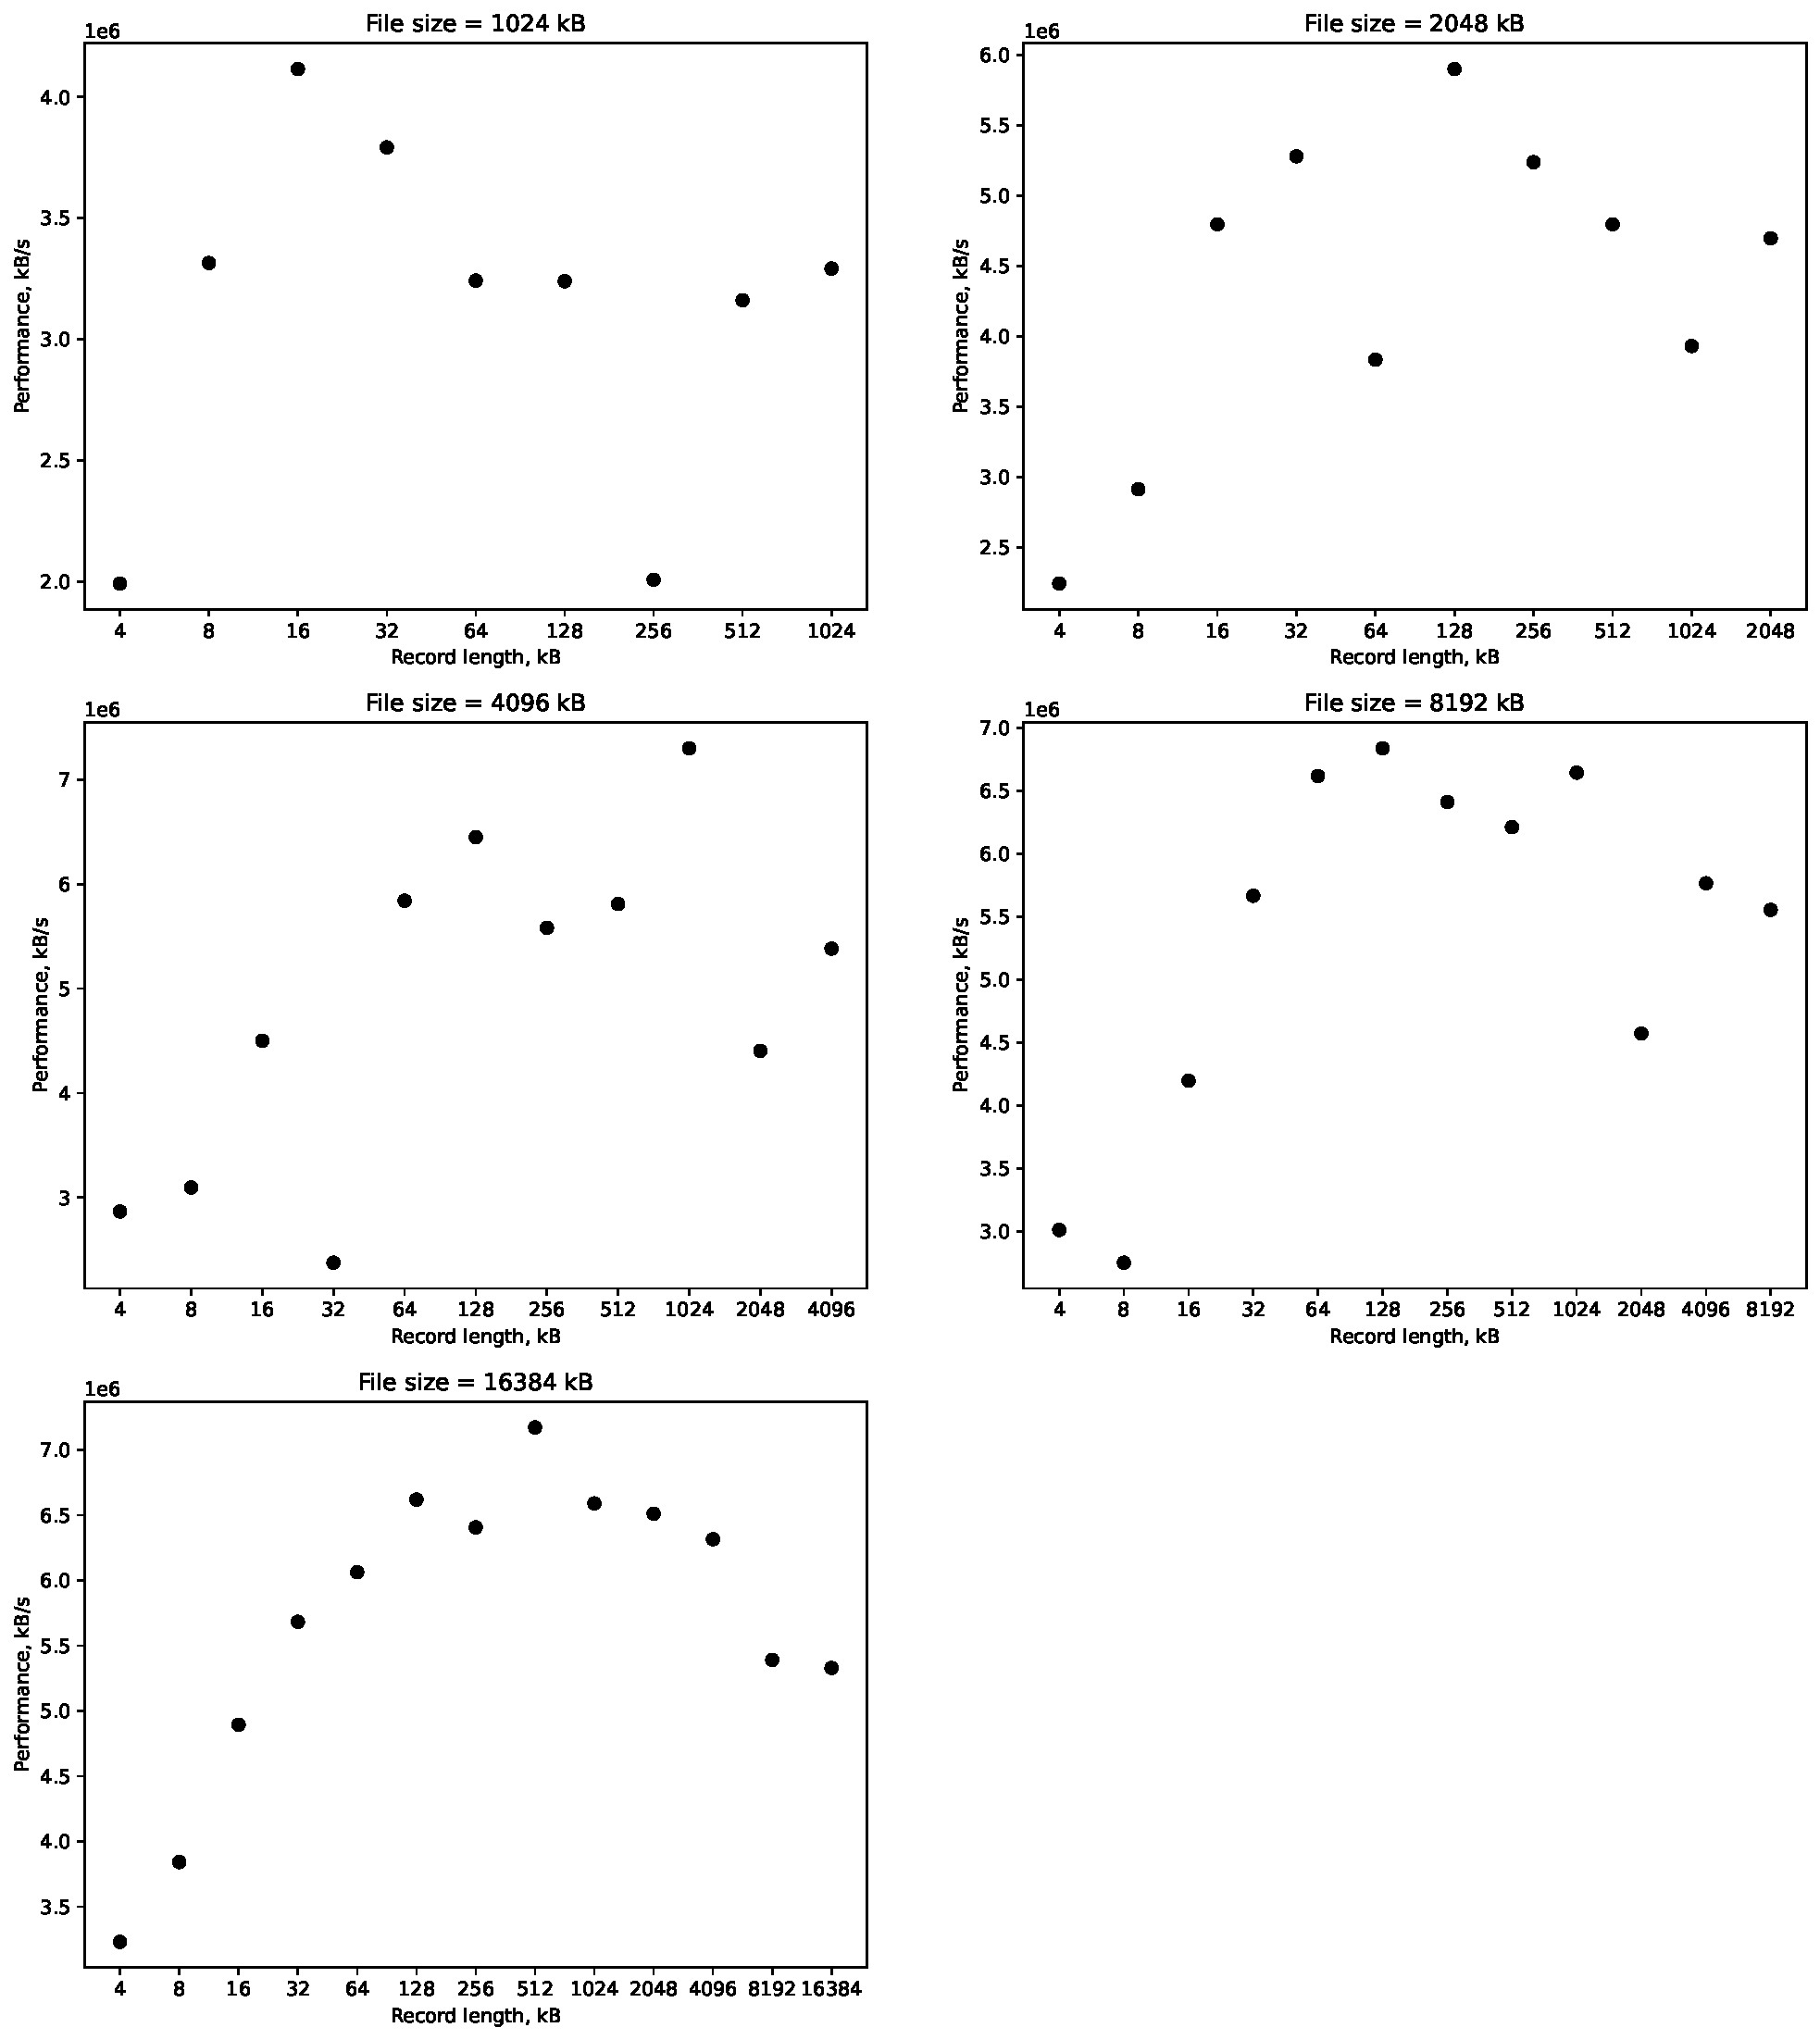
\includegraphics[width=1.0\textwidth]{figures/benchmarking/fake-ffs/Reader.pdf}
	\end{center}
	\caption{IOZone output for Fake FFS Forward Read}
\end{figure}

\begin{figure}[!htb]
	\label{fig:app_bench_fffs_rnd_read}
	\begin{center}
		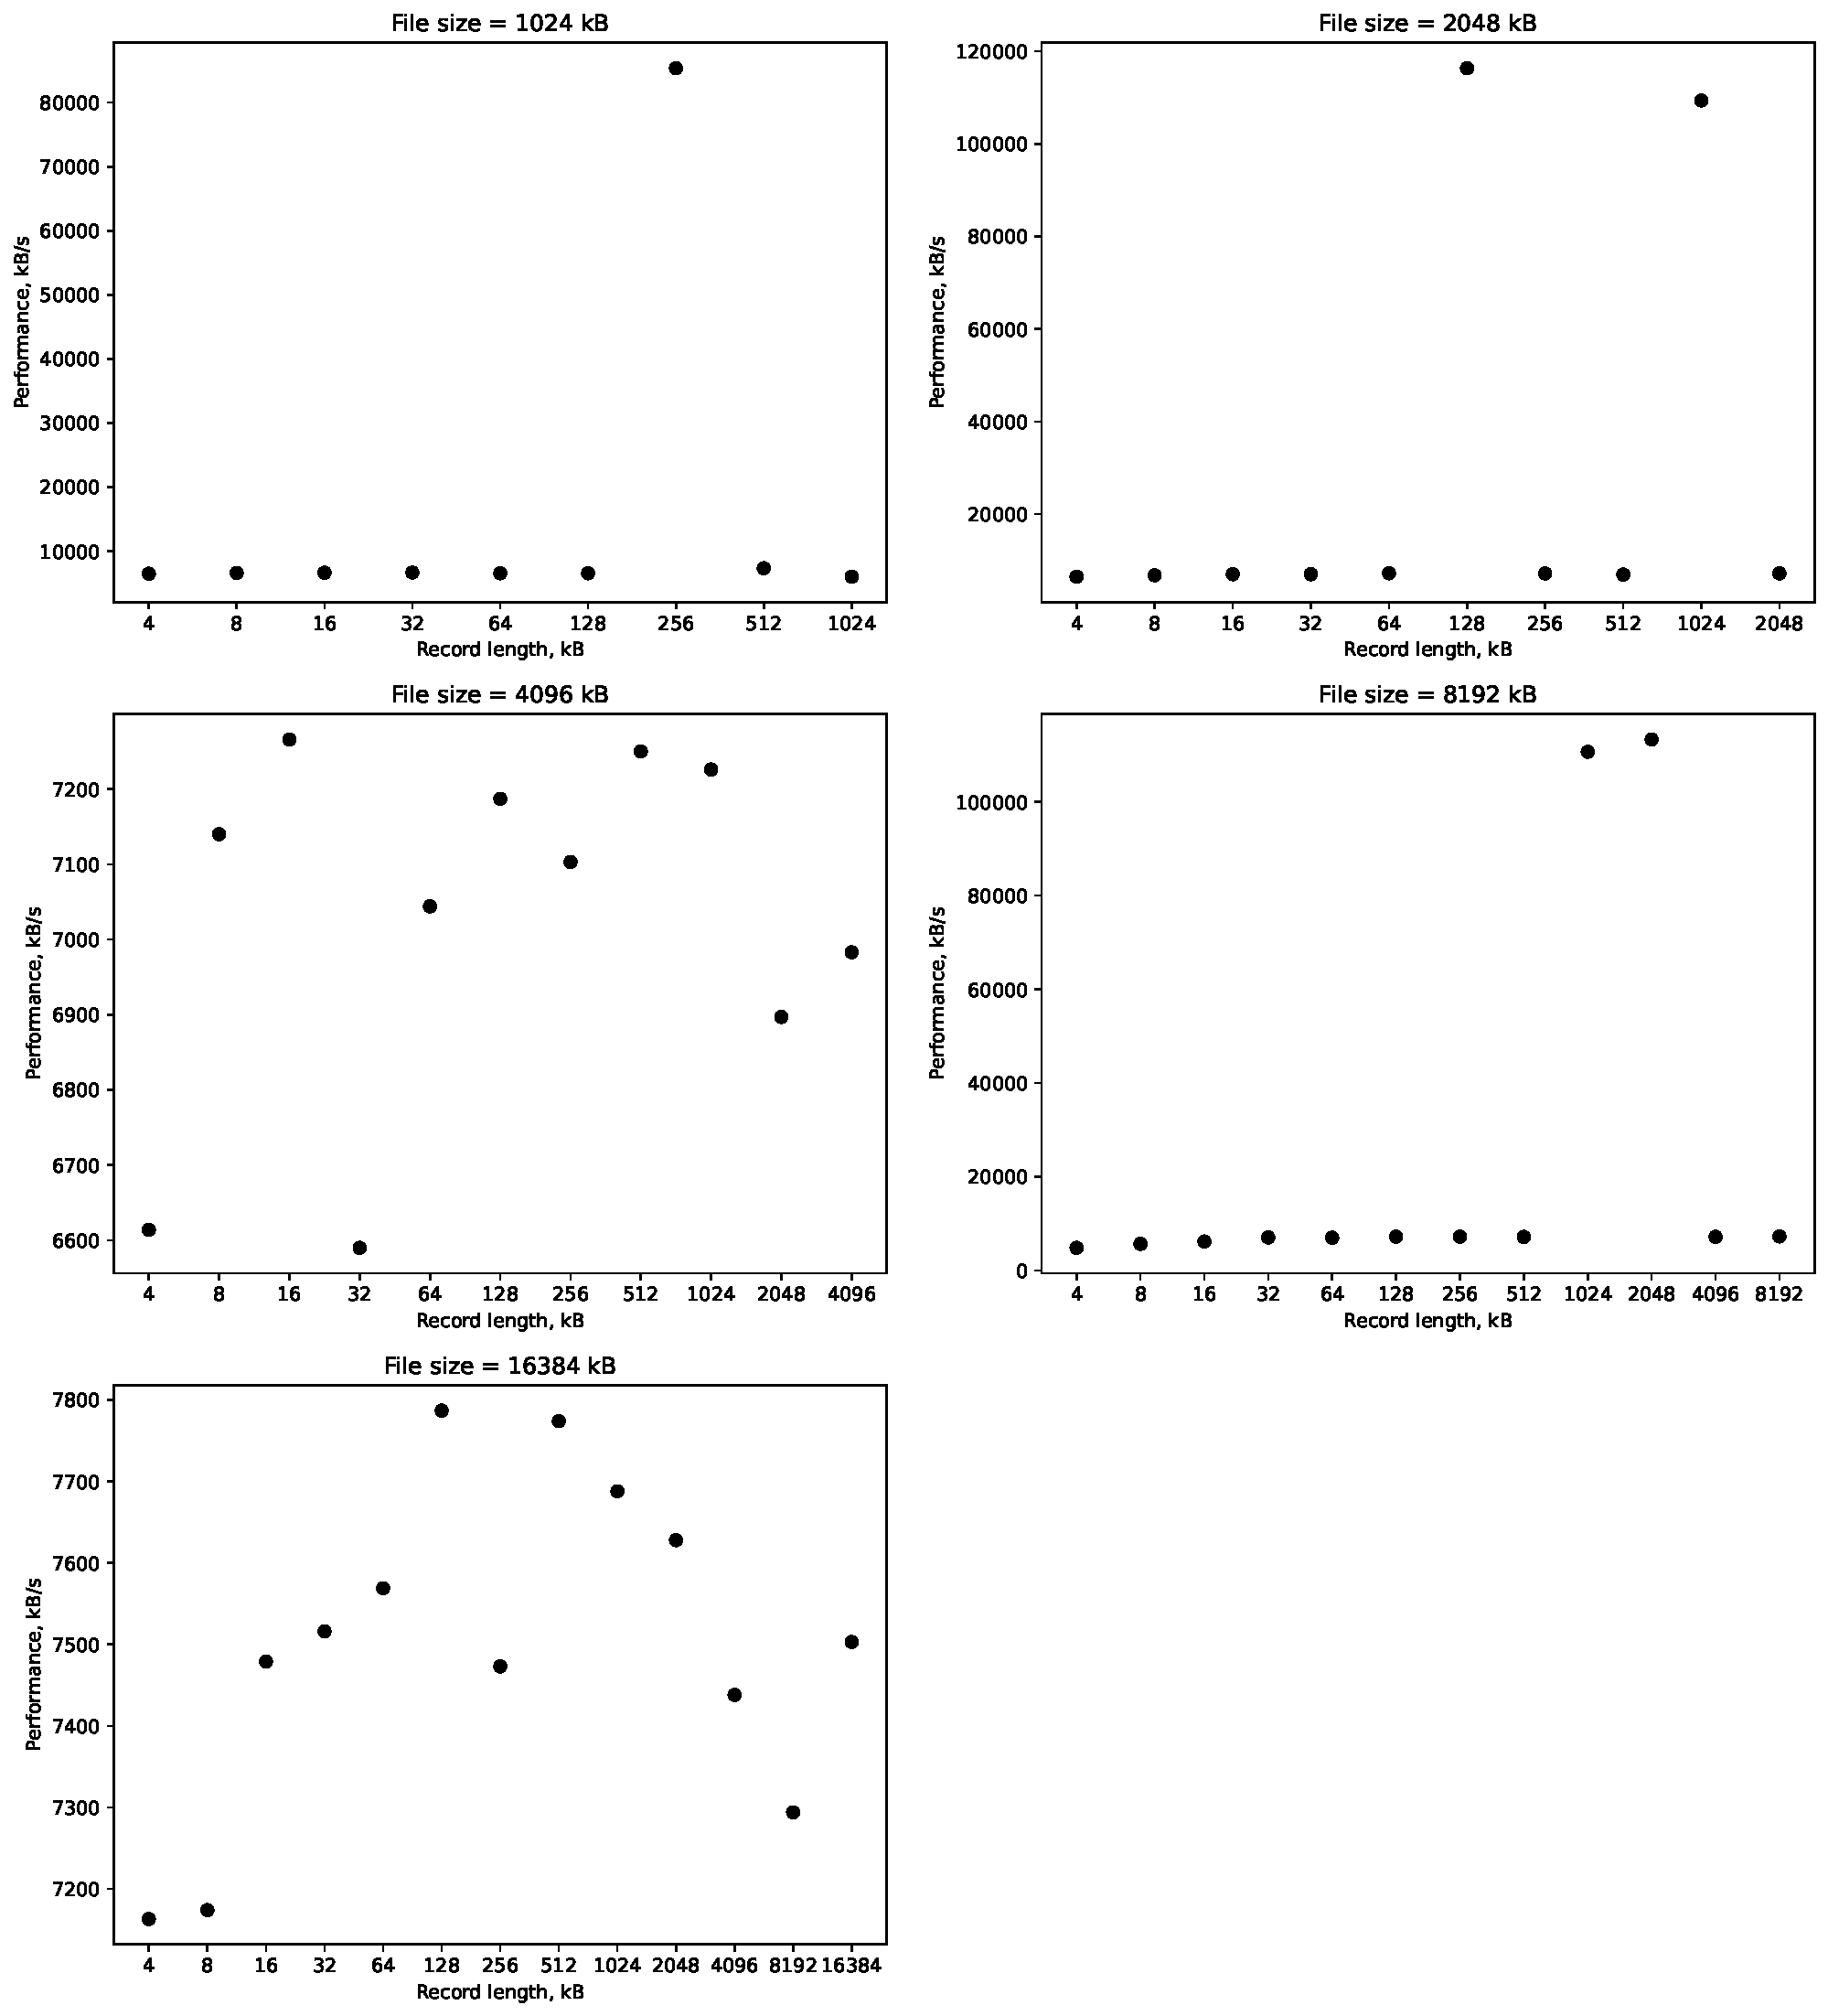
\includegraphics[width=1.0\textwidth]{figures/benchmarking/fake-ffs/Writer.pdf}
	\end{center}
	\caption{IOZone output for Fake FFS Forward Write}
\end{figure}

\begin{figure}[!htb]
	\label{fig:app_bench_fffs_rnd_read}
	\begin{center}
		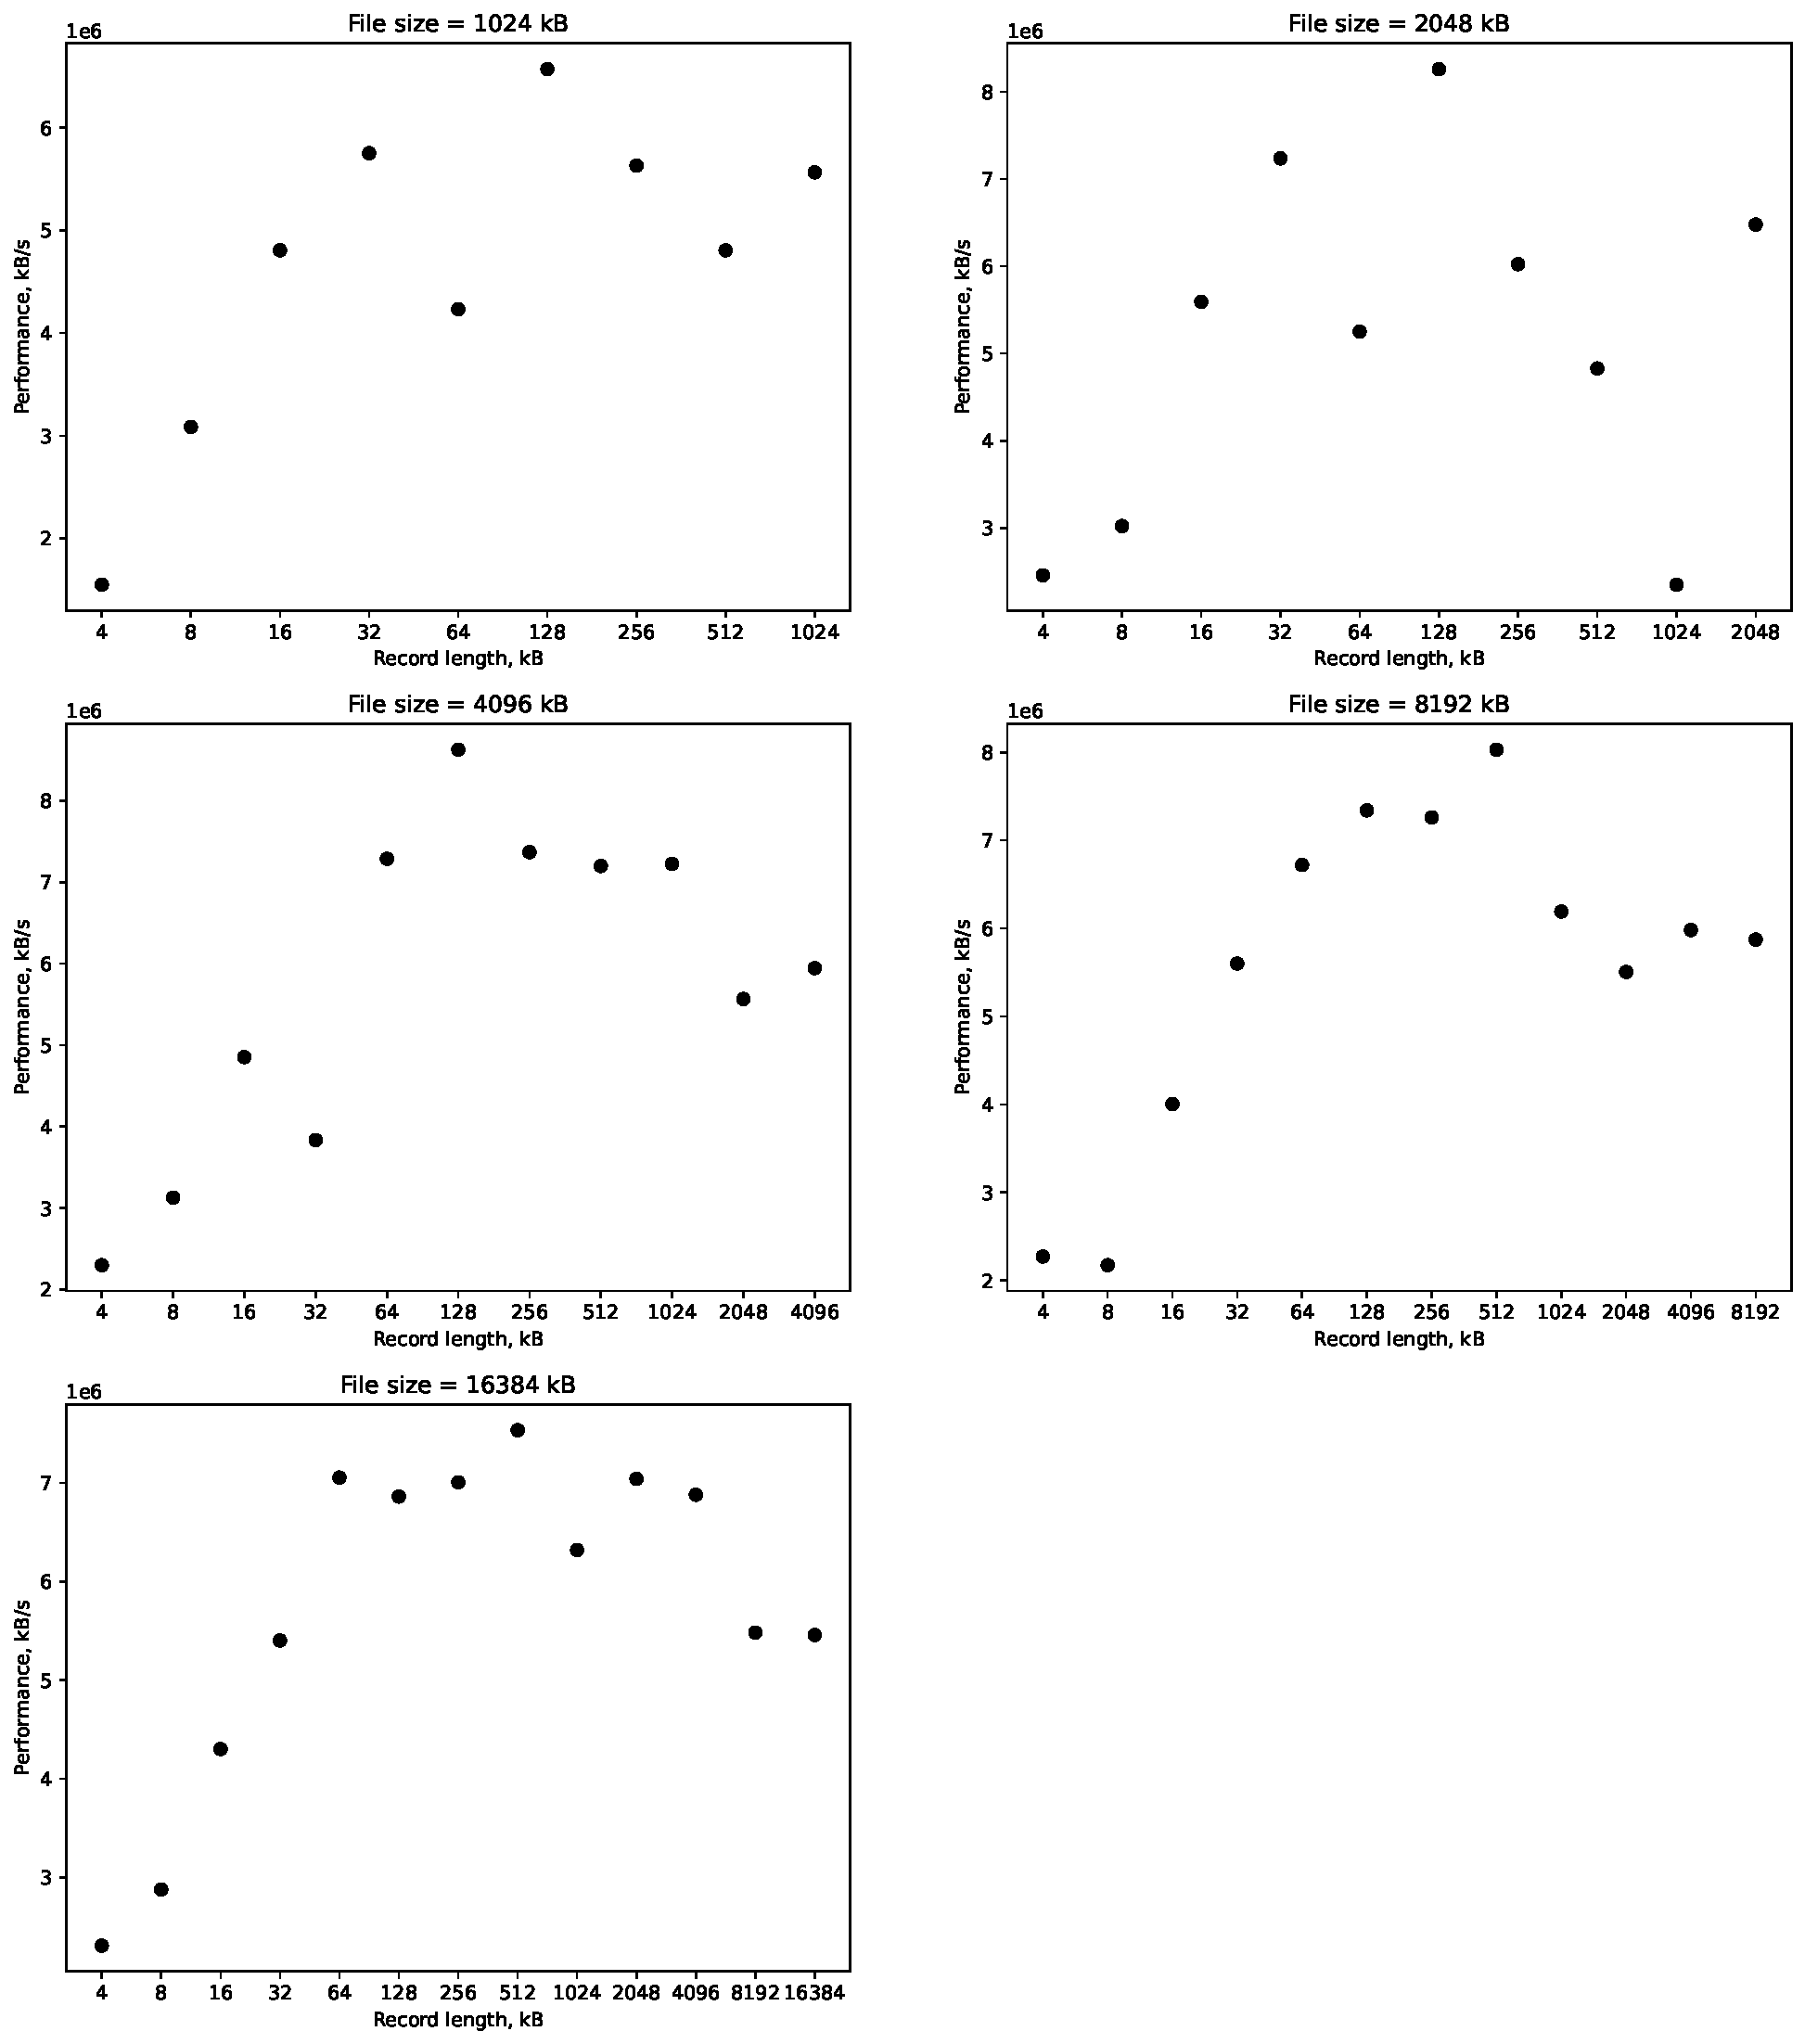
\includegraphics[width=1.0\textwidth]{figures/benchmarking/fake-ffs/Random read.pdf}
	\end{center}
	\caption{IOZone output for Fake FFS Random read}
\end{figure}

\begin{figure}[!htb]
	\label{fig:app_bench_fffs_rnd_read}
	\begin{center}
		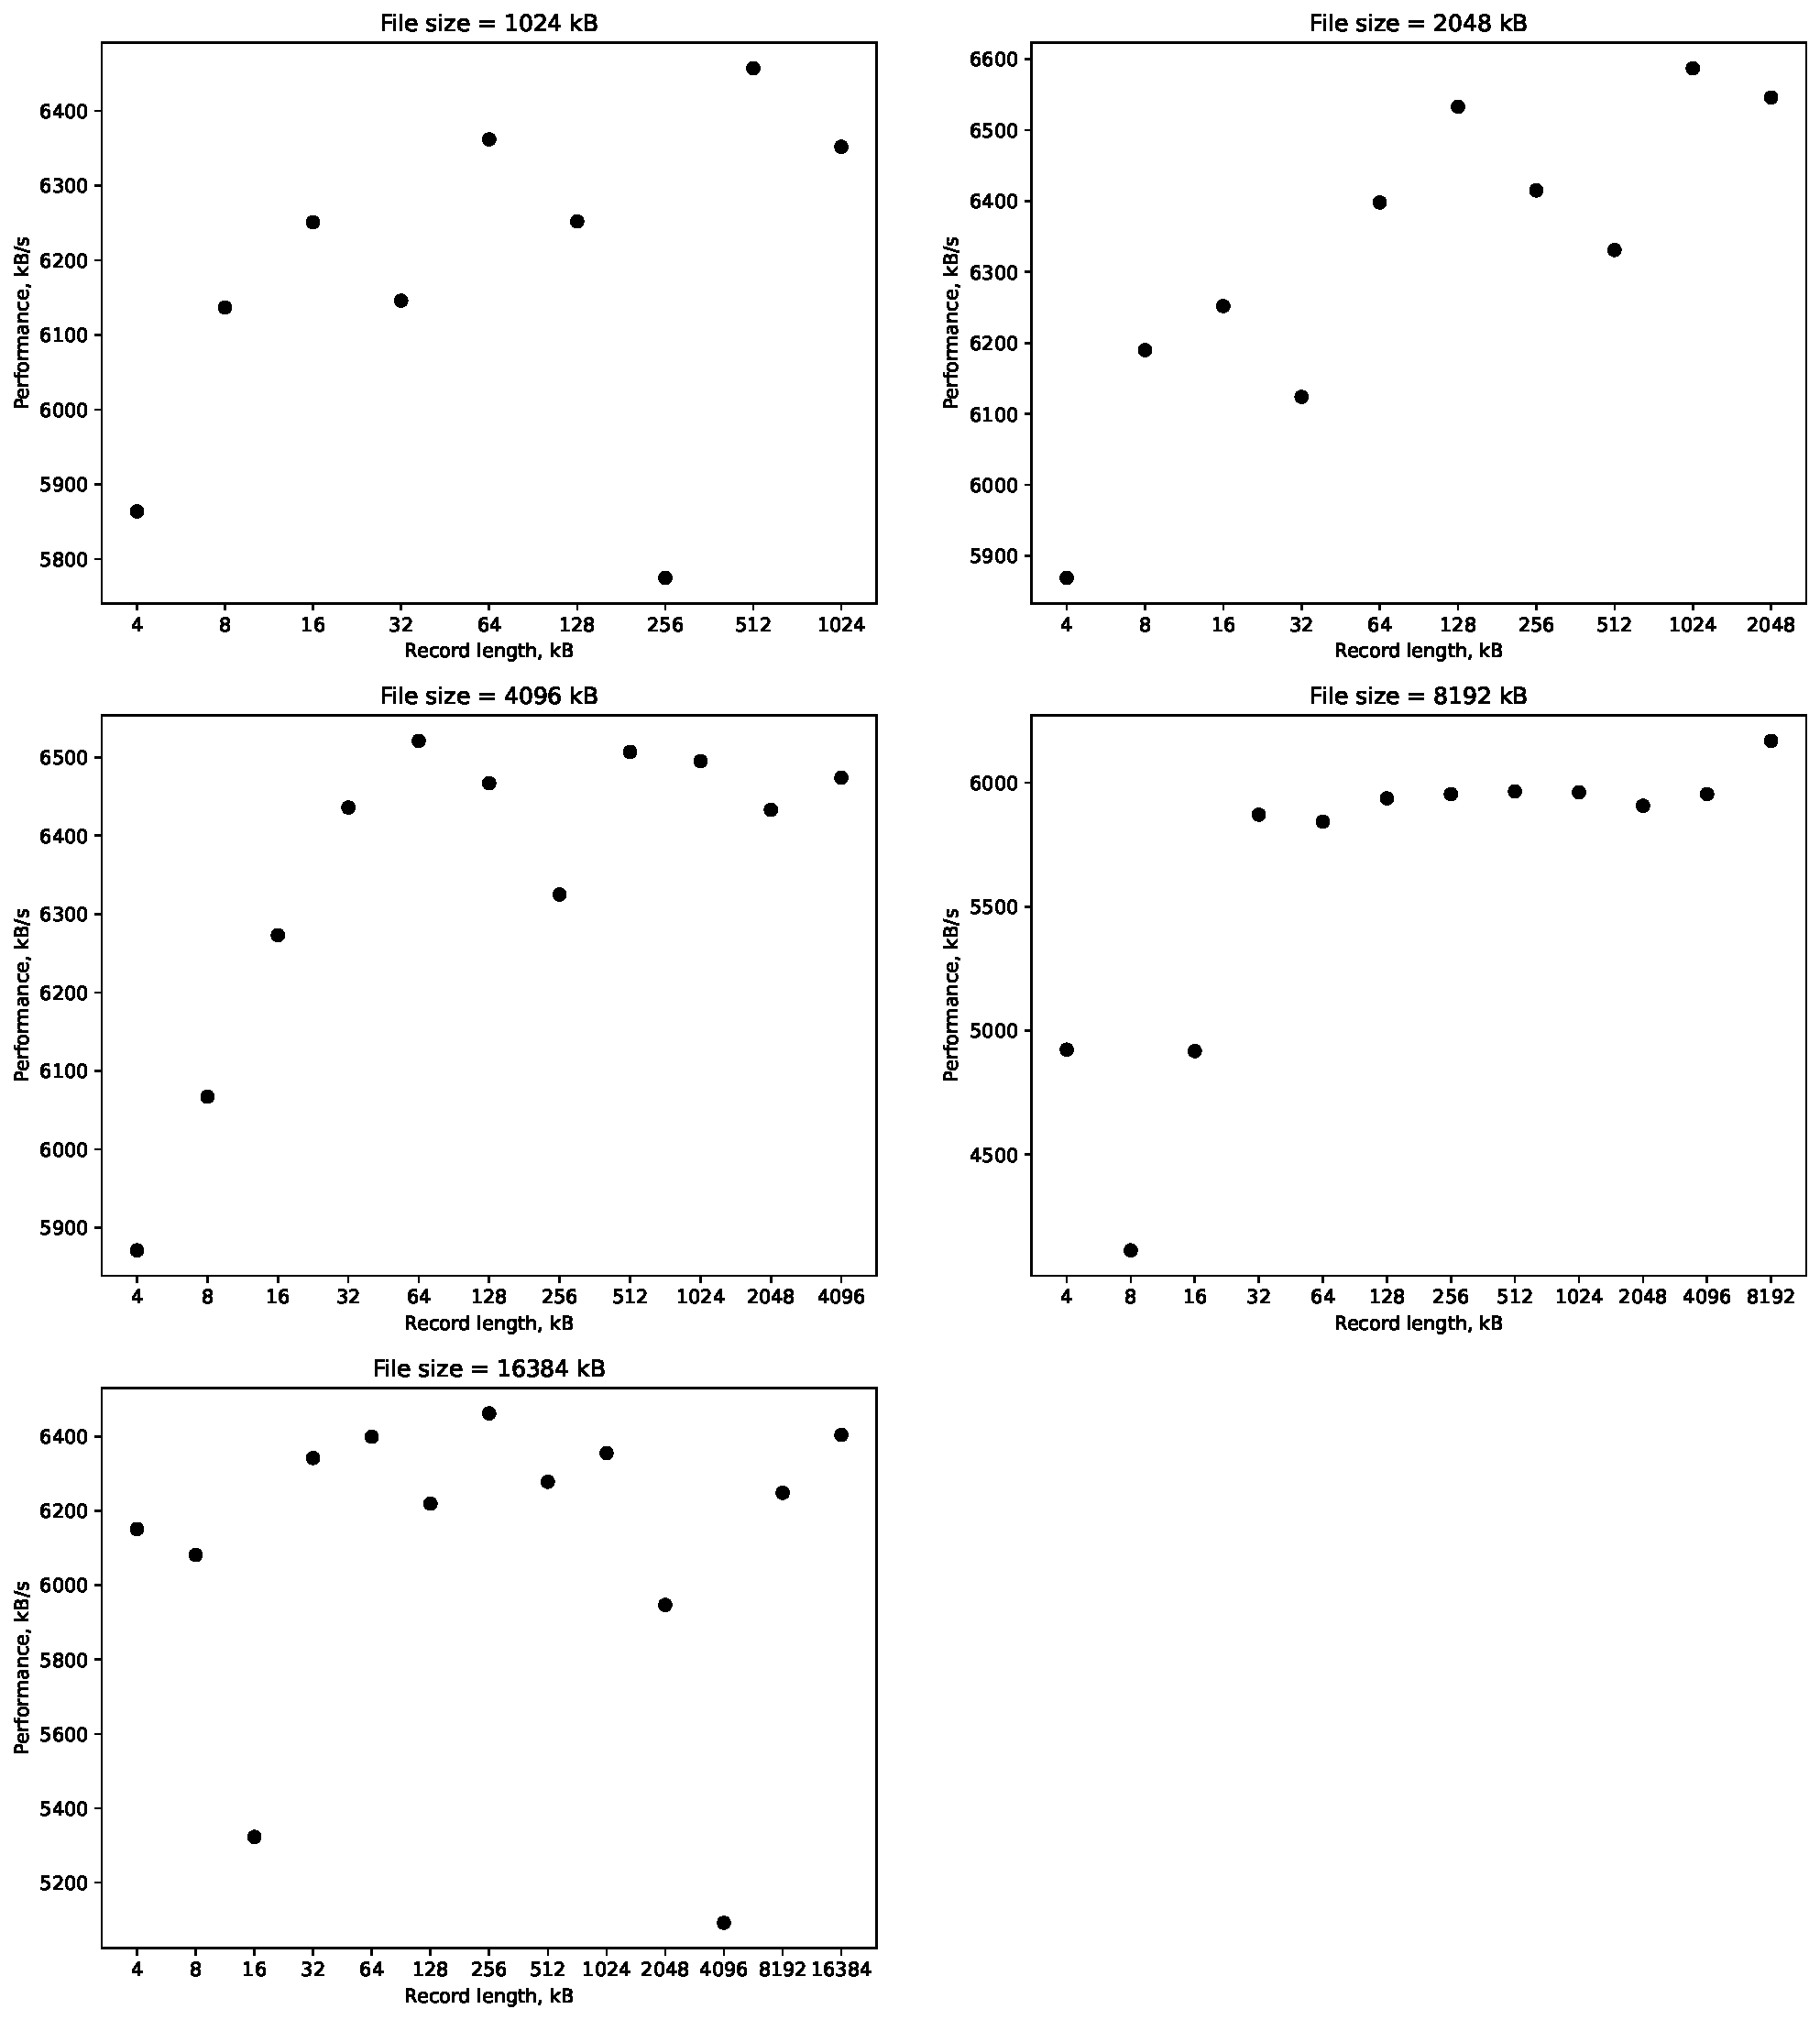
\includegraphics[width=1.0\textwidth]{figures/benchmarking/fake-ffs/Random write.pdf}
	\end{center}
	\caption{IOZone output for Fake FFS Random write}
\end{figure}

\begin{figure}[!htb]
	\label{fig:app_bench_fffs_rnd_read}
	\begin{center}
		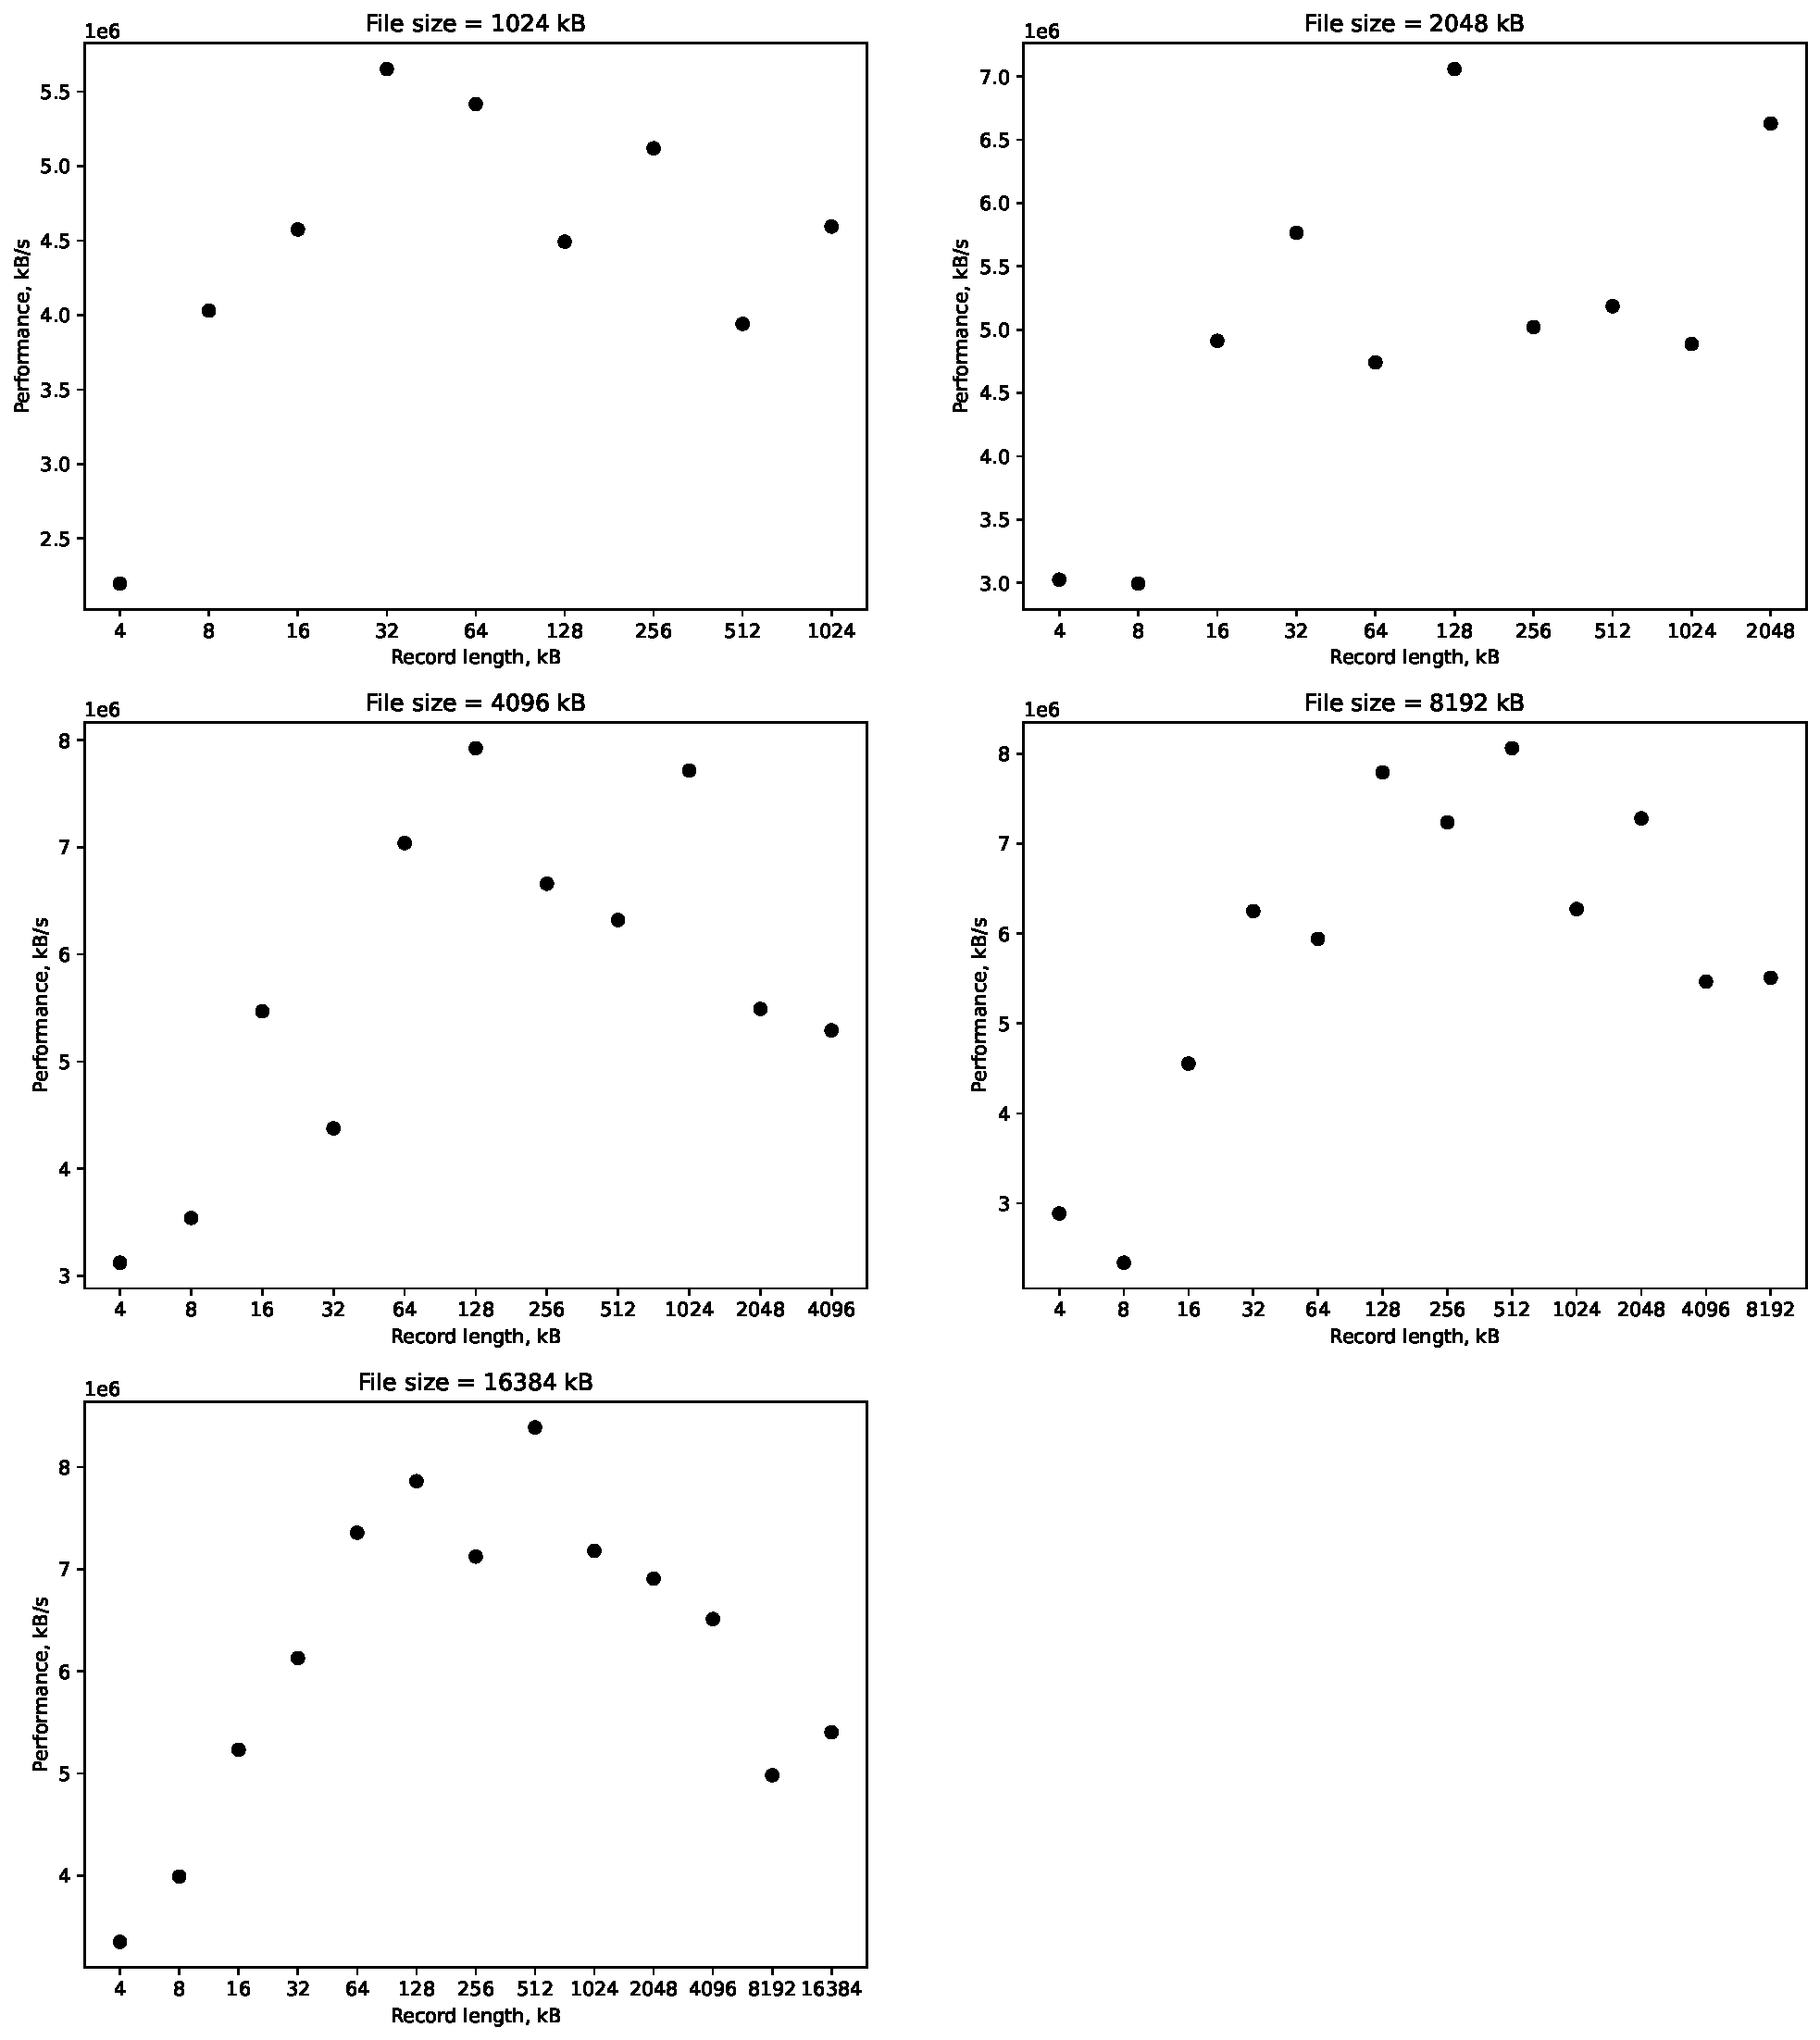
\includegraphics[width=1.0\textwidth]{figures/benchmarking/fake-ffs/Re-Reader.pdf}
	\end{center}
	\caption{IOZone output for Fake FFS Re-Read}
\end{figure}

\begin{figure}[!htb]
	\label{fig:app_bench_fffs_rnd_read}
	\begin{center}
		\includegraphics[width=1.0\textwidth]{figures/benchmarking/fake-ffs/Re-Writer.pdf}
	\end{center}
	\caption{IOZone output for Fake FFS Re-Write}
\end{figure}

\section{APFS}
\begin{figure}[!htb]
	\label{fig:app_bench_apfs_rnd_read}
	\begin{center}
		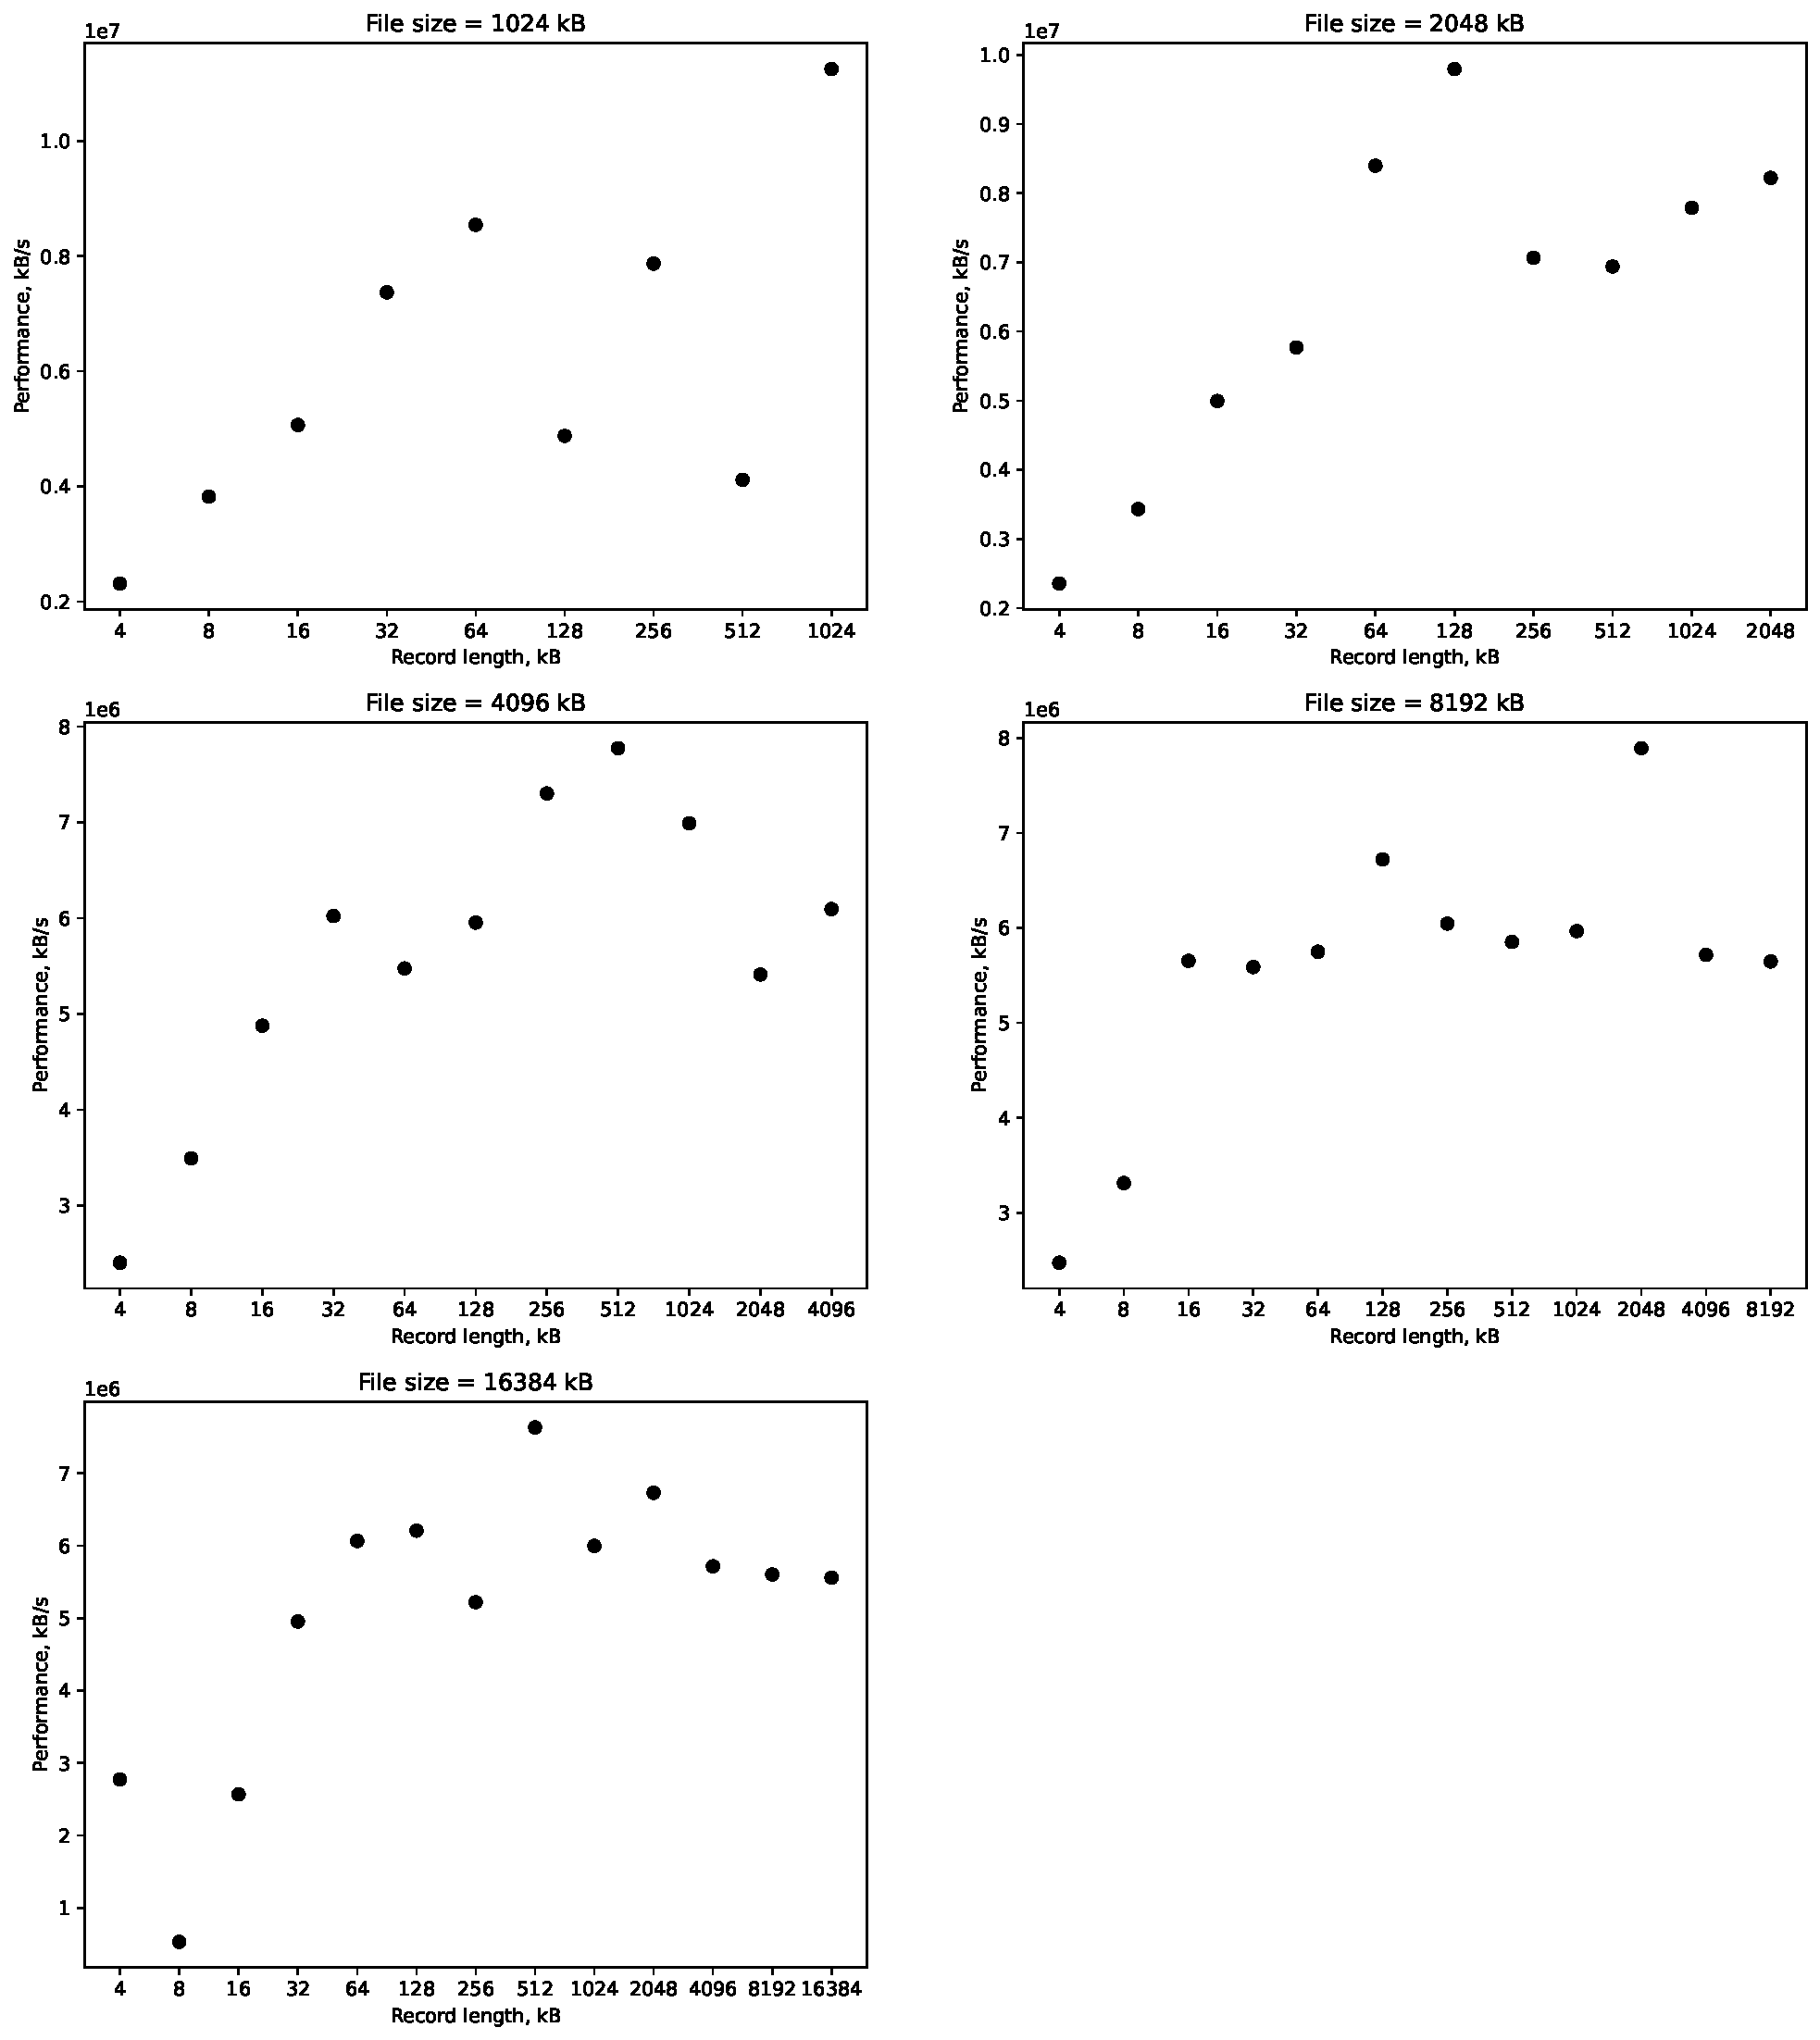
\includegraphics[width=1.0\textwidth]{figures/benchmarking/local/Reader.pdf}
	\end{center}
	\caption{IOZone output for APFS Forward Read}
\end{figure}

\begin{figure}[!htb]
	\label{fig:app_bench_apfs_rnd_read}
	\begin{center}
		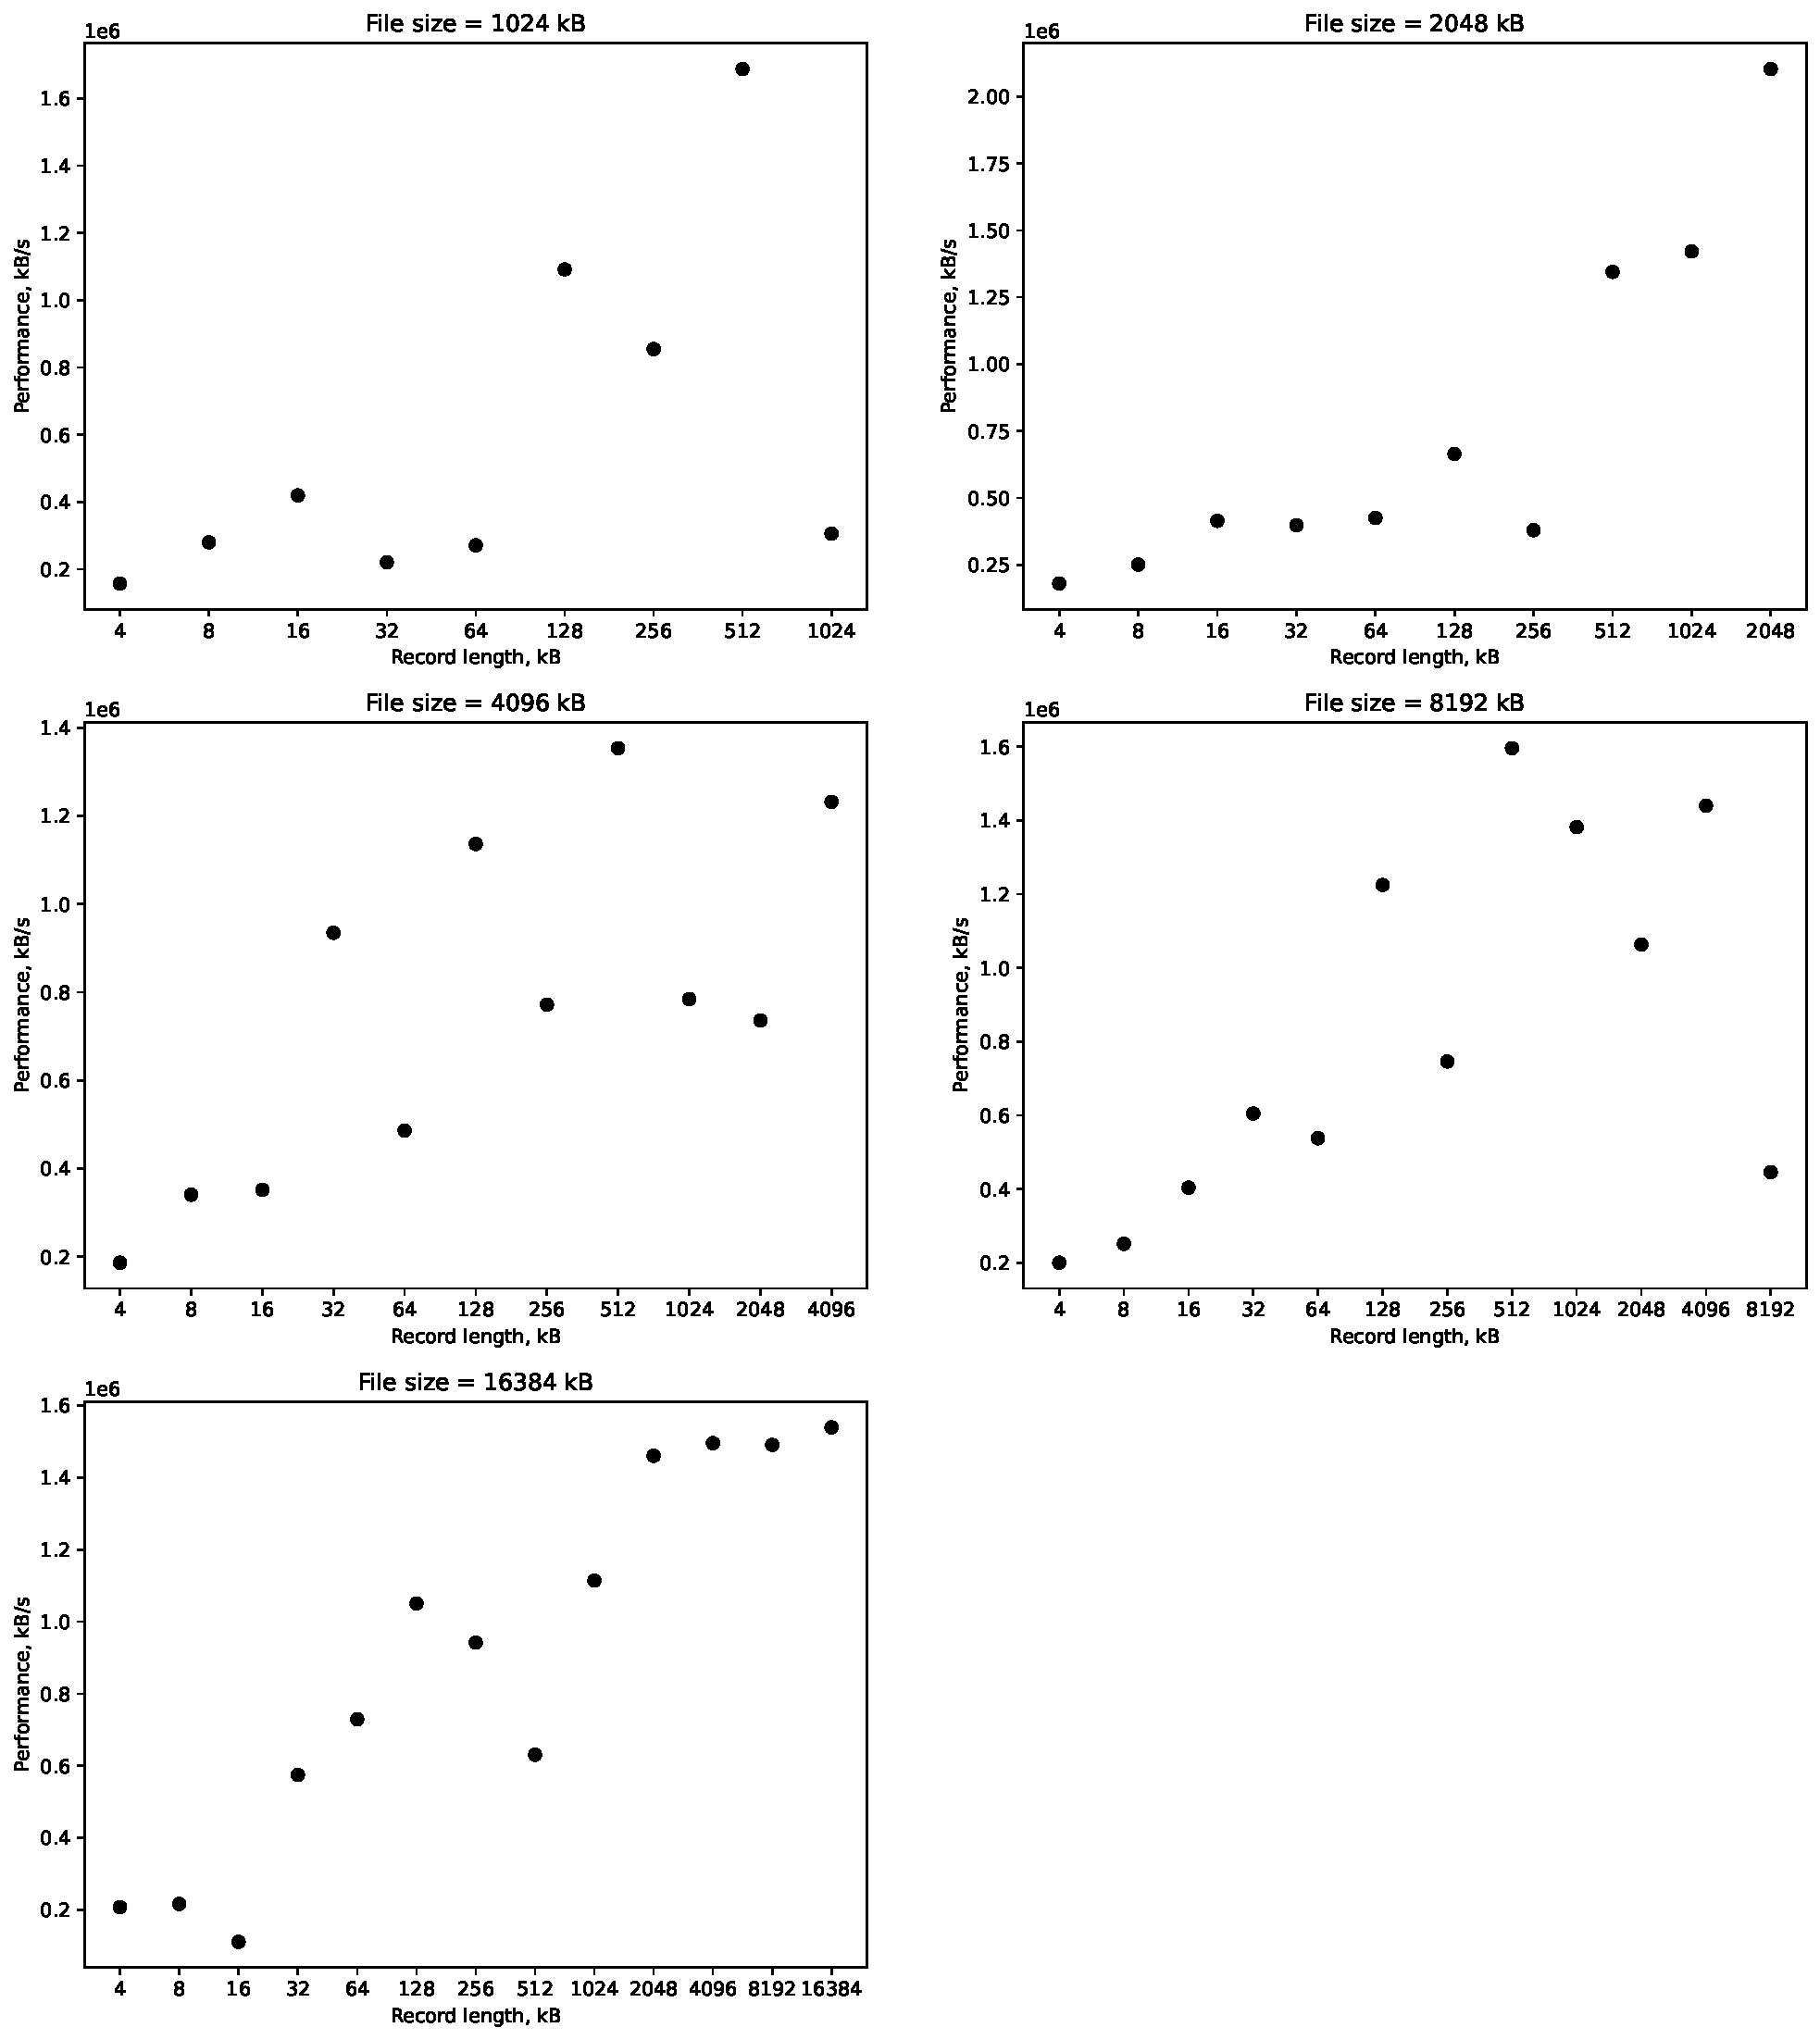
\includegraphics[width=1.0\textwidth]{figures/benchmarking/local/Writer.pdf}
	\end{center}
	\caption{IOZone output for APFS Forward Write}
\end{figure}

\begin{figure}[!htb]
	\label{fig:app_bench_apfs_rnd_read}
	\begin{center}
		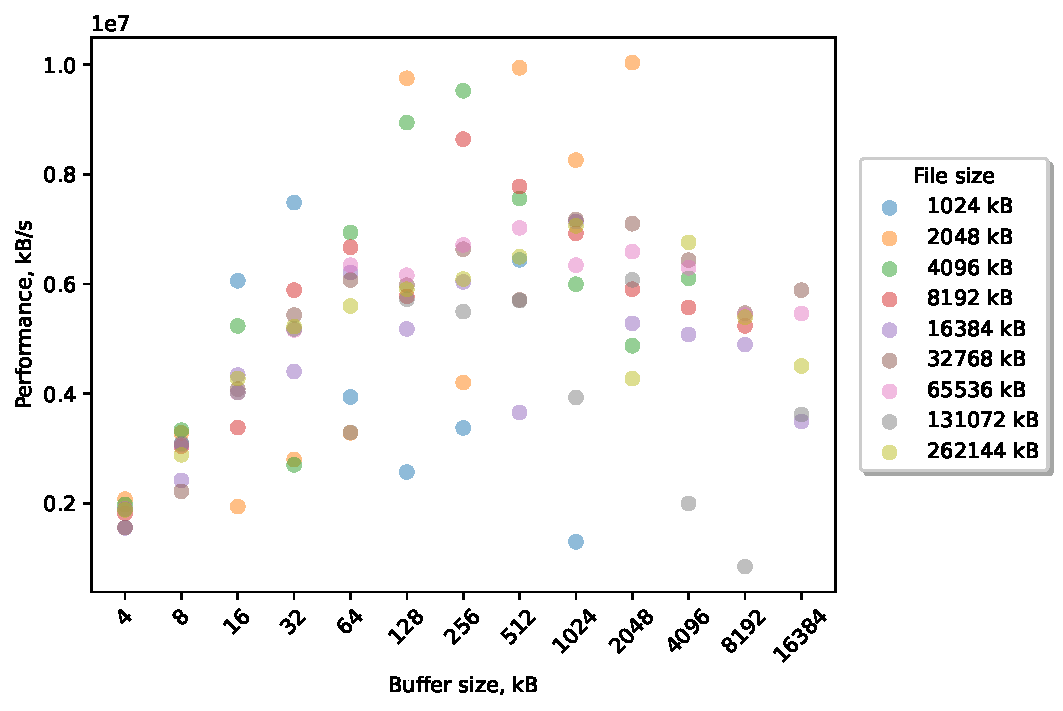
\includegraphics[width=1.0\textwidth]{figures/benchmarking/local/Random read.pdf}
	\end{center}
	\caption{IOZone output for APFS Random read}
\end{figure}

\begin{figure}[!htb]
	\label{fig:app_bench_apfs_rnd_read}
	\begin{center}
		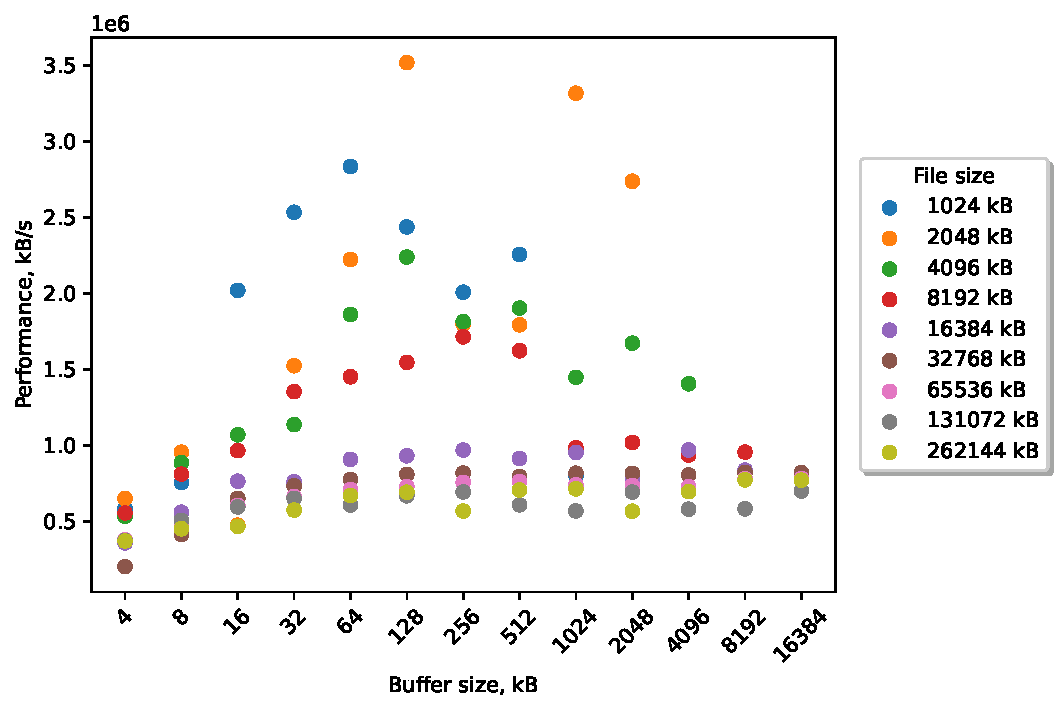
\includegraphics[width=1.0\textwidth]{figures/benchmarking/local/Random write.pdf}
	\end{center}
	\caption{IOZone output for APFS Random write}
\end{figure}

\begin{figure}[!htb]
	\label{fig:app_bench_apfs_rnd_read}
	\begin{center}
		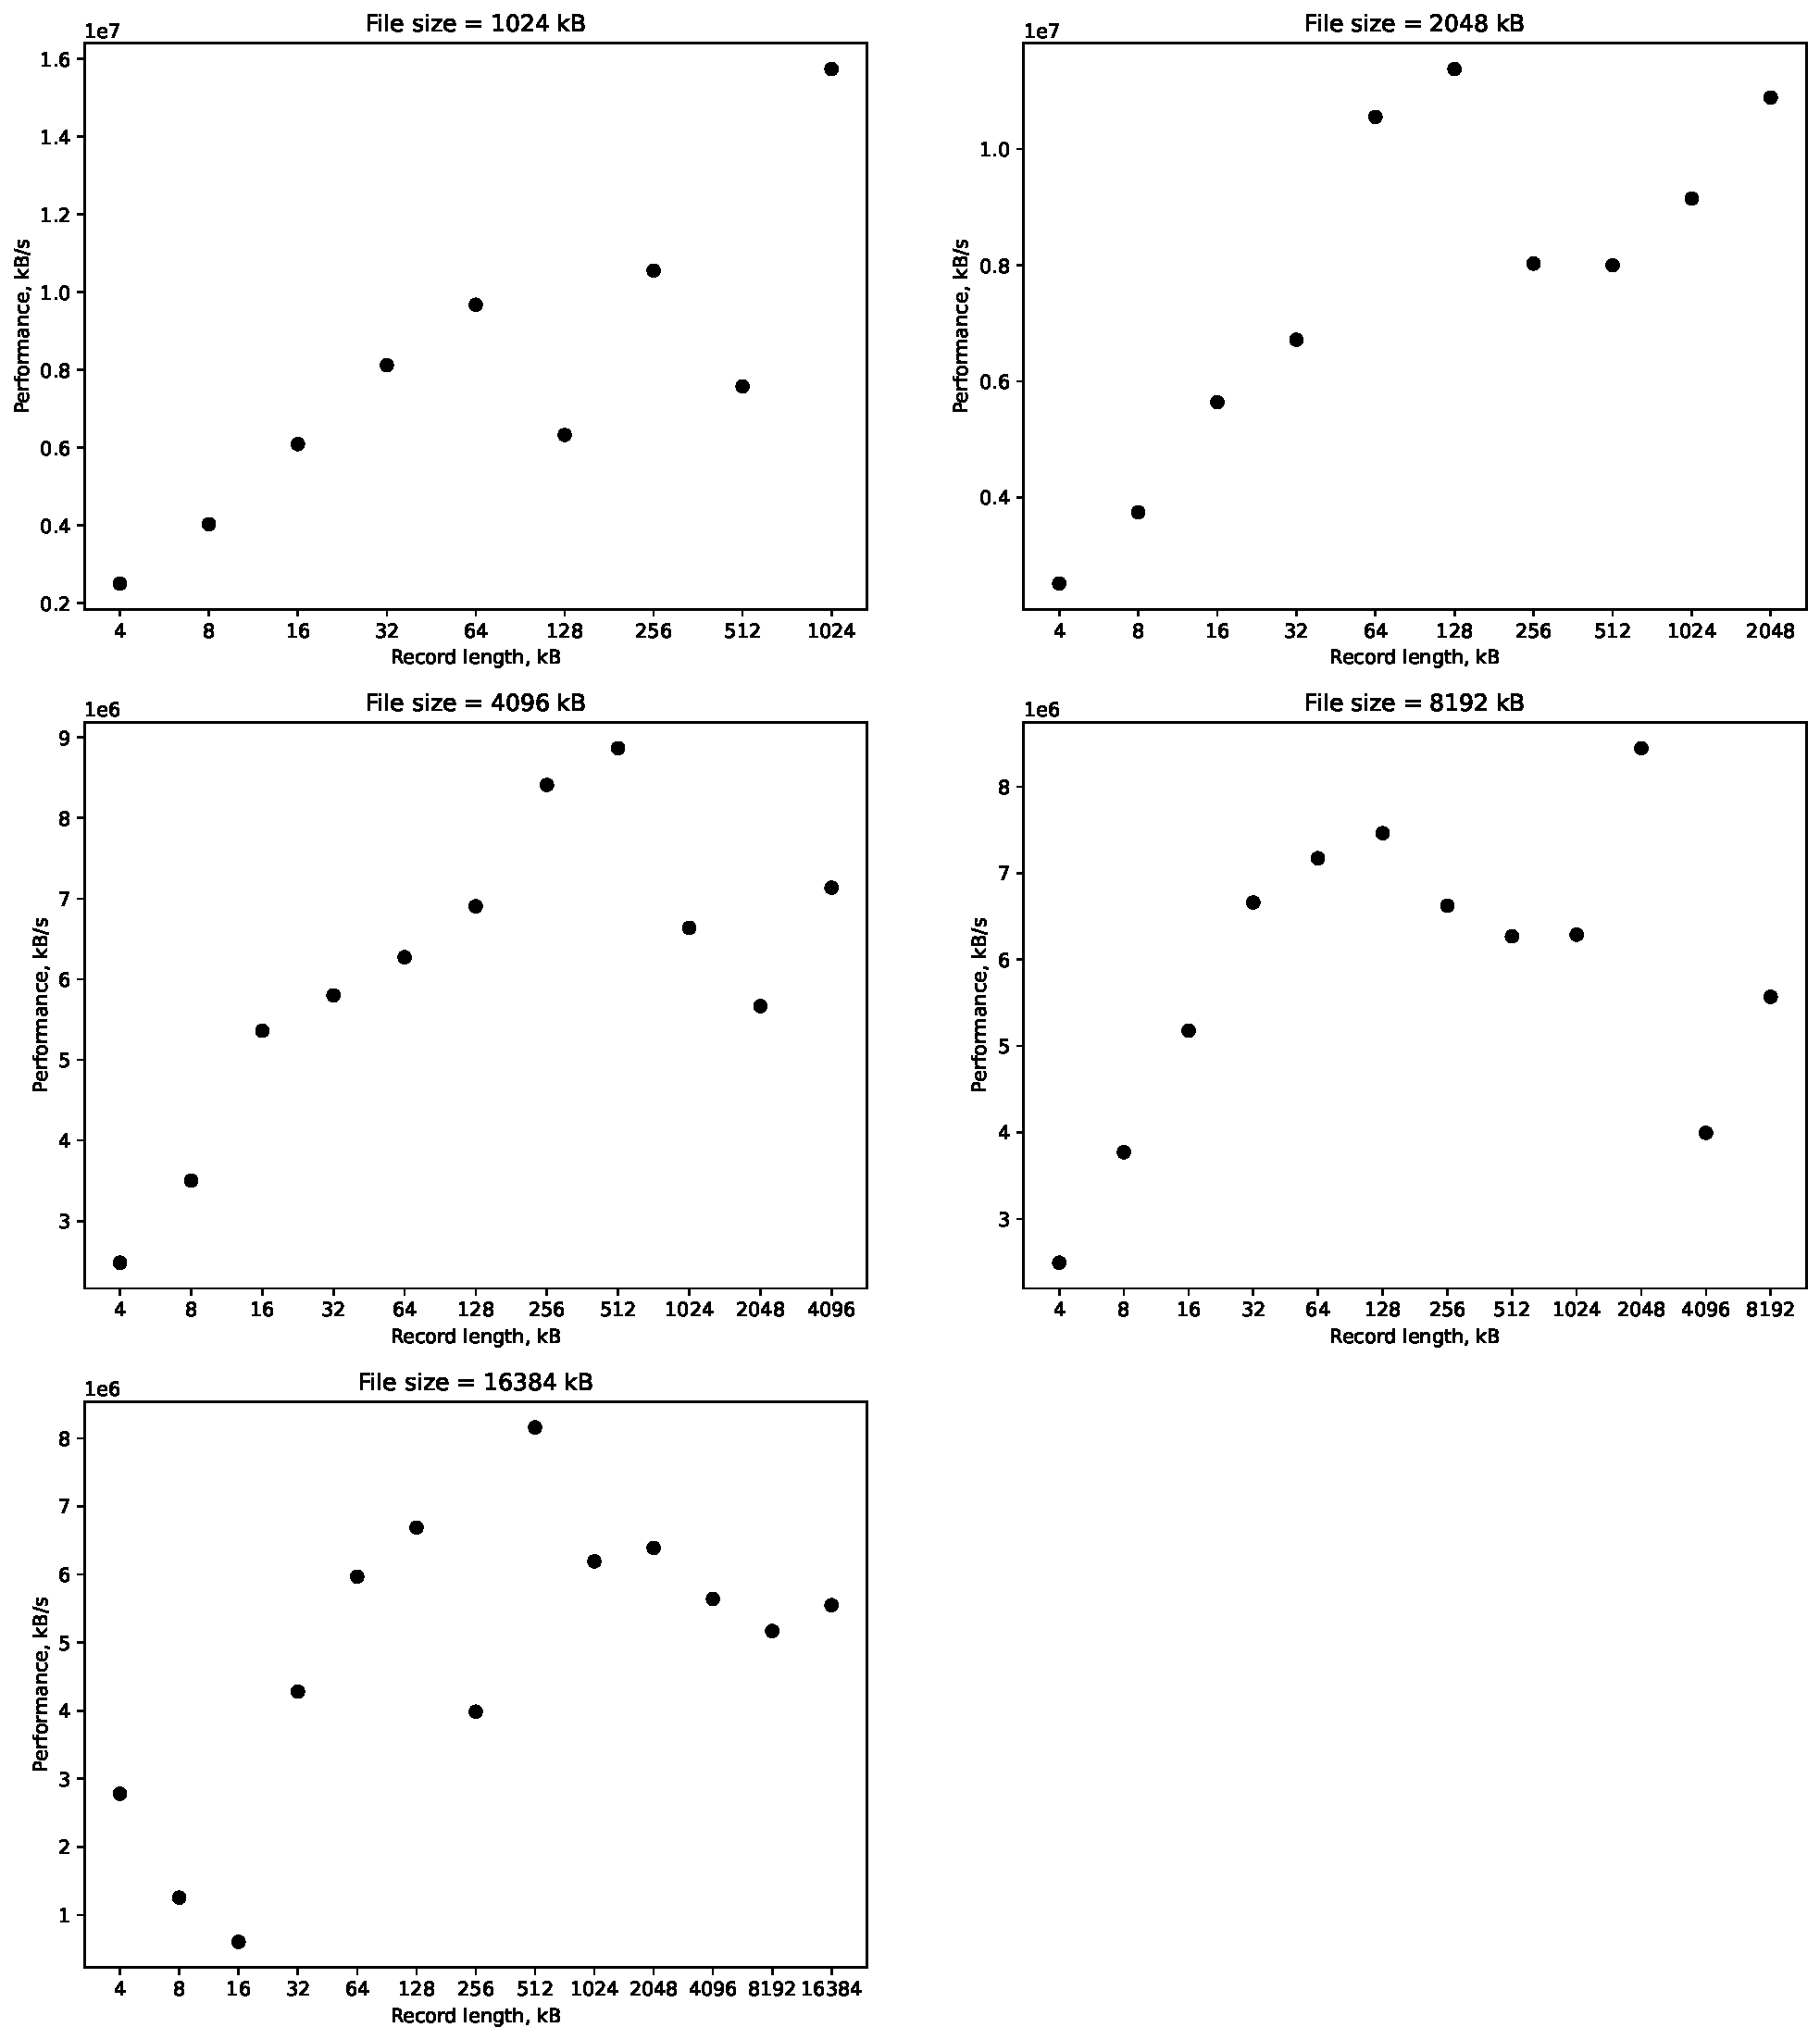
\includegraphics[width=1.0\textwidth]{figures/benchmarking/local/Re-Reader.pdf}
	\end{center}
	\caption{IOZone output for APFS Re-Read}
\end{figure}

\begin{figure}[!htb]
	\label{fig:app_bench_apfs_rnd_read}
	\begin{center}
		\includegraphics[width=1.0\textwidth]{figures/benchmarking/local/Re-Writer.pdf}
	\end{center}
	\caption{IOZone output for APFS Re-Write}
\end{figure}